s%Metodología
\section{Metodología}

\begin{figure}[H]
  \centering
  \adjustbox{width = 15cm}{
\ctikzsubcircuitdef{power}{in 1,in 3,in 2}{
    coordinate (#1-in 1) to[R,l=$R_{17}$,*-*] ++(0,-4.50) coordinate (#1-in 3)
    (#1-in 3) --++(1.5,0) node[npn,anchor=B](Q5){$Q_{5}$}
    (#1-in 1) -| (Q5.C)
    (Q5.E) to[R,l=$R_{13}$,*-*] ++(0,-2) coordinate (A) to[C,l_=$C_{5}$] ++(2,0) to[R,l=$R_{L}$,*-*] ++(0,-2) node[vee](VEE){$-10\volt$}
    (A) to[R,l=$R_{14}$,*-*] ++(0,-2) node[pnp, anchor=E](Q6){$Q_{6}$}
    (#1-in 3) --++(0,-1.5) coordinate(A1) --++(1,0) --++ (0,-0.5) node[npn,anchor=C](Q4){$Q_{4}$}
    (Q4.E) --++(0,-0.5) --++(-1,0) coordinate(A2)
    (A1) --++(-1,0) --++(0,-0.71) node[potentiometershape, rotate=-90,anchor=west,label=south west:$R_{V1}$, font=\large](P){}
    (P.wiper) -| (Q4.B)
    (P.east) --++(0,-0.71) -| (A2)
    (A2) --++(0,-1.5) coordinate (A3) -| (Q6.B)
    (A3) to[R,l=$R_{12}$,*-] ++(0,-2) coordinate (#1-in 2)
    (Q6.C) --++(0,-1.5) -| (#1-in 2)
}

\ctikzsubcircuitdef{driver}{in 1, in 2, in 3, out 1, out 2, out 3}{
coordinate (#1-in 3) --++(0.5,0) node[pnp, anchor=B](Q3){$Q_{3}$}
(#1-in 3) to[R,l=$R_{15}$,*-*] ++(0,3.23) coordinate (#1-in 1) ++(0,0) node[vcc](VCC){$10\volt$}
(#1-in 3) --++(0,-1.27) coordinate (B1) to[R,l=$R_{10}$,*-*] ++(0,-7.81) coordinate (#1-in 2) ++(0,0) node[vee](VEE){$-10\volt$}
(Q3.E) to[R,l=$R_{11}$,*-*] ++(0,2.46) coordinate (B3)
(Q3.E) --++(1.5,0) to[C,l=$C_{6}$,*-*] ++(0,2.46) coordinate (#1-out 1) --(B3) -| (#1-in 1)
(Q3.C) --++(0,-0.5) coordinate (#1-out 3) to[R,l=$R_{16}$,*-*] ++(0,-7.81) coordinate (#1-out 2) -| (#1-in 2)
(B1) --++(0.4,0) to[C,l=$C_{4}$] ++(0.5,0) -| (#1-out 3)
}

\ctikzsubcircuitdef{differential}{in 1,out 1, out 2,out 3}{
    coordinate (#1-in 1) --++(1,0) node[npn, anchor=B](Q1){$Q_{1}$}
    (Q1.C) --++(0,1) coordinate (#1-out 3) to[R,l=$R_{3}$,*-] ++(0,2) coordinate (C)
    (Q1.E) to[R,l=$R_{4}$,*-] ++(0,-6) coordinate (C2)
    (#1-in 1) to[R,l=$R_{1}$,*-*] ++(0,5) -| (C)
    (#1-in 1) to[R,l=$R_{2}$,*-*] ++(0,-7.31) -| (C2)
    (Q1.E) to[R,l_=$R_{5}$,*-*] ++(2.5,0) coordinate (C3) to[R,l=$R_{7}$,*-*] ++(0,-6.54) coordinate (C6) -| (C2)
    (C3) node[npn,xscale=-1, anchor=E,label=left:$Q_{2}$](Q2){} ++(0,1.5)
    (Q2.C) to[R,l=$R_{6}$,*-*] ++(0,4.23) coordinate (C4) -| (C)
    (Q2.B) --++(0.5,0) coordinate (C5) to[R,l=$R_{9}$,*-*] ++(0,-7.31) coordinate (#1-out 2) -| (C6)
    (C5) to[R,l=$R_{8}$,*-*] ++(0,5) coordinate (#1-out 1) -| (C4)
    (C5) --++(1,0) to[C,l=$C_{3}$,*-*] ++(0,-2) node[vee](VEE){$-10\volt$}
}
\ctikzsubcircuitdef{universall}{in 1,out 3}{
    coordinate (#1-in 1) --++(1,0) node[npn, anchor=B](Q1){$Q_{1}$}
    (Q1.C) --++(0,1) coordinate (#1-out 3) to[R,l=$R_{3}$,*-] ++(0,2) coordinate (C)
    (Q1.E) to[R,l=$R_{4}$,*-] ++(0,-6) coordinate (C2)
    (#1-in 1) to[R,l=$R_{1}$,*-*] ++(0,5) -| (C)
    (#1-in 1) to[R,l=$R_{2}$,*-*] ++(0,-7.31) -| (C2) (Q1.E) 
}

\ctikzsubcircuitactivate{universall}
\ctikzsubcircuitactivate{power}
\ctikzsubcircuitactivate{driver}
\ctikzsubcircuitactivate{differential}

\begin{circuitikz}\draw
    (0,0)\driver{driv}{out 3} to[C,l=$C_{7}$,*-*]++(3,0) \power{power}{in 3}
    (driv-out 1) -| (power-in 1)
    (driv-out 2) -| (power-in 2)
    (driv-in 3) to[C,l=$C_{2}$,*-*]++(-6,0) \differential{dif}{out 3}
    (driv-in 1) -| (dif-out 1)
    (driv-in 2) -| (dif-out 2)
    (dif-in 1) to[C,l=$C_{1}$,*-*] ++(-2,0) to[short,-o, label=$V_{in}$] ++(-0.5,0)
;\end{circuitikz}
}
  \caption{Diagrama Esquemático del Amplificador Base}
  \label{fig:amplificador_base}
\end{figure}

\subsection{Parte 1. Amplificador de potencia}
\begin{enumerate}
  \item \textbf{Identifique la etapa de Potencia (EP) en el amplificador base.}

        \begin{figure}[H]
          \centering
          \adjustbox{width = 3cm}{
\begin{circuitikz}\draw
   \power{power}{in 3}
    (driv-out 1) -| (power-in 1) ++(0,0) node[vcc](VCC){$10\volt$}
    (driv-out 2) -| (power-in 2) ++(0,-0.25) node[vee](VEE){$-10\volt$}
    (0,0) to[C,l=$C_{7}$,*-*]++(-2,0) 
;\end{circuitikz}}
          \caption{Diagrama Esquemático de la  etapa de potencia}
          \label{fig:amplificador_potencia}
        \end{figure}

        La etapa de Potencia es la que se observa en la figura \ref{fig:amplificador_potencia}, que se ve reflejada también en la figura \ref{fig:amplificador_base} como última etapa del amplificador base.

  \item \textbf{Determinar los puntos de reposo de todos los transistores
          en la EP.}

        En esta etapa, los transistores  $Q_5$ y $Q_6$ son complementarios (es decir, uno es de tipo NPN y otro PNP), debido    a no estar ensamblados bajo la misma oblea de silicio, ambos podrían tener una ganancia distinta, pudiéndose encontrar algunas diferencias, al estar polarizado en su zona activa.

        Se trabajaran de manera ideal, por esta razón, los puntos de operación o reposo de los transistores son iguales para ambos.

        Donde se encuentra la resistencia $R_{v1}$ y el transistor $Q_4$, se conoce como \textbf{Multiplicador de voltaje base-emisor}. Este nos permite mantener una caída de tensión entre base-emisor de los transistores $Q_5$ y $Q_6$ de $0.65\volt$.

        \subsubsection{Análisis DC}
        En esta oportunidad del análisis en DC, despreciamos las corrientes de base de ambos transistores, por ser pequeñas y que la corriente que pasa por $R_{17}$ es aproximadamente $I_{EQ5}$.

        Esto último es consecuencia de que entre el multiplicador Base-Emisor y el punto de salida $V_o$, debe existir idealmente una caída de tensión de $V=0 \, V$, por esta razón, se indica que $I_{R_{17}}=I_{EQ_5}$, más adelante se detalla este tema.

        Ahora, Aplicando Ley de Corrientes de Kirchhoff (LCK), se obtiene lo siguiente:

        \begin{equation}
          I_{R_{17}}=I_{R_{V1}}+I_{CQ4}
          \label{eqn:ir17}
        \end{equation}

        Como se indica anteriormente su corriente en base es despreciable.

        Si aplicamos Ley de Ohm, tenemos que,


        \begin{align}
          {V_{CEQ_4}} & =I_{R_{V1}}\cdot R_{V1} \nonumber          \\[0.2cm]
          I_{R_{V1}}  & =\dfrac{V_{CE}}{R_{V1}} \label{eqn:ir17_3}
        \end{align}
        Esta corriente, se toma en cuenta con la caída de tensión de Base-Emisor

        \begin{align}
          I_{R_{V1}} & =\dfrac{V_{BEQ_4}}{xR_{V1}} \label{eqn:ir17_2}
        \end{align}

        Si se igualan las ecuaciones \ref{eqn:ir17_3} y \ref{eqn:ir17_2}, se obtiene la siguiente expresión:

        \begin{align}
          \dfrac{V_{CEQ_4}}{R_{V1}} & =\dfrac{V_{BEQ_4}}{xR_{V1}} \nonumber                                       \\[0.2cm]
          V_{CEQ_4}                 & = \dfrac{V_{BEQ_4}\cdot R_{V1} }{xR_{V1}} = \dfrac{V_{BEQ_4} }{x} \nonumber \\[0.2cm]
          V_{CEQ_4}                 & =\dfrac{V_{BEQ_4} }{x} \label{eqn:vce}
        \end{align}

        Donde, $x \in [0,1]$, para que los transistores $Q_5$ y $Q_6$, se encuentren al borde de la conducción si y solo si el voltaje de colector-emisor sea 2 veces el $V_{BEQ_5}$ o $V_{BEQ_6}$ \, ; debido a la tensión que se halla entre base y emisor.

        Con este análisis se tiene que $x=\dfrac{1}{2}$, debido a la demostración siguiente, sustituyendo $x$ en la ecuación \ref{eqn:vce}:

        \begin{align}
          V_{CE} & =\dfrac{V_{BE} }{\dfrac{1}{2}} = 2 V_{BEQ_5}= 2 V_{BEQ_6}\label{eqn:vce2}
        \end{align}

        Siendo $x$, el valor que se le dara a la resistencia variable para obtener la ecuación \ref{eqn:vce2}

        Tomando el valor de $R_{V1}=10k \therefore xR_{V1}=\dfrac{10k}{2} =5k \Omega$

        Aplicando Leyes de Voltaje de Kirchhoff, haciendo un recorrido por las resistencias $R_{17}, R_{V1}$ y $R_{12}$, sabiendo $I_{R_{17}}={I_{EQ_5}}$

        \begin{align*}
          10+10-I_{R_{17}}\cdot 22k-V_{CEQ_4} -I_{R_{12}}\cdot 22k = 0 \\[0.2cm]
          I_{R_{17}}= \dfrac{20-2 V_{BEQ_5}}{44k}=\dfrac{20-2 (0.65)}{44k}=425 \mu A
        \end{align*}

        \begin{align}
          I_{EQ_5} & =I_{EQ_6}=425 \mu A
          \label{eqn:ieq5}
        \end{align}

        Luego se despeja de la ecuación \ref{eqn:ir17}, $I_{CQ_4}$ y sustituimos el valor de la ecuación \ref{eqn:ir17_2} y \ref{eqn:ieq5}, tenemos:

        \begin{align}
          I_{R_{17}} & =I_{R_{V1}}+I_{CQ_4} \nonumber       \\[0.2cm]
          I_{CQ_4}   & = I_{R_{17}}-I_{R_{V1}} \nonumber    \\[0.2cm]
          I_{CQ_4}   & = 425 \mu-\dfrac{0.65}{5k} \nonumber \\[0.2cm]
          I_{CQ_4}   & = 295 \mu A \label{eqn:icq4}
        \end{align}

        Idealmente los valores de $I_{CQ_5}$ e $I_{CQ_6}$ es cero pero como ambos no son totalmente ideal por lo explicado en el principio del apartado, se tiene que $I_{CQ_5}$ e $I_{CQ_6}$ si poseen una pequeña corriente que tomar en cuenta.

        Por otro lado, se puede comprobar que idealmente da cero, como se demuestra a continuación:

        Aplicando LVK en la malla donde se encuentran los tres transistores, se tiene:

        \begin{align*}
          -V_{BEQ_5}-I_{E_5}(10+10)-V_{BEQ_4} + -V_{CEQ_4} =0 \\[0.2cm]
          I_{E_5} = \dfrac{V_{CEQ_4}-2V_{BEQ_5}}{20}=\dfrac{2V_{BEQ_5}-2V_{BEQ_5}}{20}=0
        \end{align*}

        Sin embargo, tomando en cuenta esa corriente se tiene lo siguiente:

        Considerando la configuración Push-Pull se activa un transistor en un ciclo y viceversa, de esa manera solo estará encendido $Q_5$, con una impedancia muy baja del multiplicador Base-Emisor (Cable o corto), donde se obtendrá una configuración universal del transistor $Q_5$, con $R_{17}$, $R_{12}$, $R_{13}$ y $R_L$.

        Se aplica superposición para hallar el $V_{th}$

        \begin{gather}
          V_{th}=V_{CC}\dfrac{R_{12}}{R_{12}+R_{17}}+V_{EE}\dfrac{R_{17}}{R_{12}+R_{17}}=0
          \label{eqn:vth1}
        \end{gather}

        \begin{gather}
          R_{th}=R_{17}|| R_{12}=11\, k \ohm \label{eqn:rth1}
        \end{gather}

        Se sustituye \ref{eqn:vth1} y \ref{eqn:rth1} en la siguiente ecuación.

        Aplicando LVK en el resultante Thevenin visto desde la base hacia afuera del transistor $Q_5$

        \begin{gather}
          I_b=\dfrac{V_{th}-V_{EE}-V_{BE}}{R_{th}+R_E(\beta + 1)} =\dfrac{10-0.65}{11\, k +2.21\, k\,  (151) } = 27.12 \mu A \label{eqn: IB1}
        \end{gather}


        Recordar que
        \begin{gather}
          I_E=I_B+I_C \label{eqn:I_E}
        \end{gather}


        Si se despeja $I_C$, se obtiene,

        \begin{gather}
          I_C = I_E - I_B \label{eqn:nodos}
        \end{gather}

        Sustituyendo \ref{eqn: IB1} y \ref{eqn:ieq5} en \ref{eqn:nodos} se tiene el resultado de $I_{CQ_5}=I_{CQ_6}$

        \begin{gather}
          I_{CQ_5}=I_{EQ_5}-I_{BQ_5}=425-27.12=397.88\, \mu A \label{icq5}
        \end{gather}


        aunque si se esta despreciando $I_B \therefore I_E=I_C$

        $$I_{CQ_5}=I_{CQ_6}=I_{E_5}=0$$

        Se aplica LVK por el recorrido de $Q_5$ y $Q_6$ y se obtiene la siguiente ecuación:

        Recuerda antes, que sí, se coloca $I_E$ en función de $I_C$, se obtiene lo siguiente:
        \begin{align*}
          I_E & =I_B+I_C=\dfrac{I_c}{\beta}+I_C=(\dfrac{1}{\beta}+1)I_C \\[0.2cm]
          I_E & =\dfrac{1+\beta}{\beta}I_C
        \end{align*}

        \begin{align*}
          10-V_{CEQ_5}-\left(\dfrac{\beta + 1}{\beta}\right )I_C(20)-V_{CEQ_6}+10=0 \\[0.2cm]
          V_{CEQ_5}=\dfrac{20-\left(\dfrac{\beta + 1}{\beta}\right)I_C(20)}{2}=9.99\volt \approx 10\volt
        \end{align*}

        \begin{table}[H] % La H nos permite ubicar la tabla en la posición JUSTA y no se nos mueva
          \centering
          \begin{tabular}{|c |c |c|} %tabla de 3 columnas, cada columna centrada. r: derecha l: izquierda; |: nos crea los separadores para las columnas
            \hline %Lïnea horizontal
            \textbf{Transistor} & $\mathbf{I_{CQ}[\mu A]}$ & $\mathbf{V_{CEQ}[\volt]}$ \\
            \hline
            4                   & 295                      & 1.3                       \\
            \hline
            5                   & 397.88                   & 10                        \\
            \hline
            6                   & -397.88                  & 10                        \\
            \hline
          \end{tabular}
          \caption{Puntos de operación teóricos de la EP}
          \label{tab:ptos_ep}
        \end{table}

        \subsubsection{Análisis en AC}
  \item \textbf{Determine el modelo dinámico a pequeña señal y a frecuencias medias de la EP, ganancia e impedancias de entrada y salida.}

        Se hace uso de las ecuaciones \ref{eqn:rpi}, \ref{eqn:gm}, \ref{eqn:ro}; y de los valores de corriente de la tabla \ref{tab:ptos_ep} de esa manera hallamos sus valores de esta etapa de potencia y para todas las distintas etapas que se analizaran en AC usaremos las mismas ecuaciones.

        Se asumirá para todos los transistores de las distintas etapas y en el amplificador base como un $\beta=150$

        Es importante resaltar que se va a asumir que cada uno de los transistores en las diferentes etapas el valor de $r_o \to \infty$, solo se tomará en cuenta $r_{pi}$ y $g_m$.

        \begin{align*}
          g_{m_5} & =g_{m_6}=\dfrac{I_{CQ_5}}{V_T}=\dfrac{397.88 \mu A}{25.851 mA} \nonumber \\[0.2cm]
          g_{m_5} & =15.40m \mho
        \end{align*}

        \begin{align*}
          r_{\pi_5} & =r_{\pi_6}=\beta \dfrac{V_T}{I_{CQ_5}}=150 \dfrac{25.851 mA}{397.88 \mu A} \nonumber \\[0.2cm]
          r_{\pi_5} & =9.75 k \ohm
        \end{align*}

        \paragraph{\textbf{Ganancia de tensión}}


        Se tomará en cuenta la resistencia de la carga $R_L$, de esa manera calculamos $A_v$, haciendo uso de la ecuación \ref{eqn:av}

        \begin{align*}
          A_v & = \dfrac{(g_{m_5}r_{\pi_5}+1)(R_{13}+R_L) \left(\dfrac{R_L}{R_{13}+R_L}\right)}{r_{\pi_5}+(g_{m_5}r_{\pi_5}+1)(R_{13}+R_L) } \nonumber \\[0.2cm]
          A_v & = \dfrac{(g_{m_5}r_{\pi_5}+1)R_L}{r_{\pi_5}+(g_{m_5}r_{\pi_5}+1)(R_{13}+R_L) }\nonumber                                                \\[0.2cm]
          A_v & = \dfrac{(151)2.2k}{9.75k+(151)(2.21k) }\nonumber                                                                                      \\[0.2cm]
          A_v & = 0.967                                                                                                                                \\[0.2cm]
        \end{align*}

        Si se observa de una manera ideal es una configuración Colector-Común, lo cual significa que es un seguidor de tensión y debería dar su ganancia igual a 1.

        \paragraph{\textbf{Impedancia de entrada}}

        \begin{align*}
          Z_{in} & = R_{17}||R_{12}||(r_{\pi_5}+(R_{13}+R_L)(g_{m_5}r_{\pi_5}+1)) \nonumber \\[0.2cm]
          Z_{in} & = 10.66\, k\ohm
        \end{align*}
        \paragraph{\textbf{Impedancia de salida}}

        \begin{align*}
          Z_{out} & = R_{13} + \dfrac{r_{\pi_5}}{g_{m_5}r_{\pi_5}+1}\nonumber \\[0.2cm]
          Z_{out} & = 74.57 \ohm
        \end{align*}

        \begin{table}[H]
          \centering
          \begin{tabular}{|c|c|c|}
            \hline
            $\mathbf{A_v}$ & $\mathbf{Z_{in}[\ohm]}$ & $\mathbf{Z_{out} [\ohm]}$ \\ \hline
            0.973          & 10.66 k                 & 74.57                     \\ \hline
          \end{tabular}
          \caption{Ganancia e impedancias teóricas de la Etapa de potencia}
          \label{tab:dinamico_ep}
        \end{table}

        \subsubsection{Simulación}
  \item \textbf{Realice la simulación de la etapa con el fin de verificar tanto los puntos de operación, como el modelo circuital a pequeña señal. Explique cualquier diferencia respecto a sus cálculos, si la hay.}


        \begin{table}[H]
          \centering
          \begin{tabular}{|c|c|c|}
            \hline
            \textbf{Tag} & \textbf{Puntos de operación} & \textbf{Unidad} \\
            \hline
            V(v\_ce5)    & 10                           & voltage         \\ \hline
            V(v\_ce4)    & 0.631574                     & voltage         \\ \hline
            V(v\_ce6)    & -10                          & voltage         \\\hline
            Ic(Q6)       & -0.000316159                 & device\_current \\\hline
            Ic(Q5)       & 0.00031664                   & device\_current \\\hline

            Ic(Q4)       & 0.000299118                  & device\_current \\\hline
          \end{tabular}
          \caption{Simulación de los puntos de operación de la EP}
          \label{tab:pto_ope_ep}
        \end{table}

        Observando la tabla \ref{tab:pto_ope_ep}, nos dan directamente los valores $I_{CQ_4}$, $I_{CQ_5}$ e $I_{CQ_6}$, sin embargo hay que calcular los valores de $V_{CE_4}$, $V_{CE_5}$ y $V_{CE_6}$.
        Haremos uso de las ecuaciones \ref{eqn:error} y  una diferencia de potencial como se observa en \ref{eqn:difvol},

        \begin{equation}
          V_{AB}=V_A-V_B
          \label{eqn:difvol}
        \end{equation}

        \begin{align*}
          V_{CE_4}=0.631574 - (-0.621002) \\[0.2cm]
          V_{CE_4}=1.2525 \approx 1.3 \, \volt
        \end{align*}

        \begin{align*}
          V_{CE_5}=10 - (0.0.00844586) \\[0.2cm]
          V_{CE_5}=9.99 \approx 10 \, \volt
        \end{align*}

        \begin{align*}
          V_{CE_6}=-10 - (0.00209375) \\[0.2cm]
          V_{CE_6}=-10.00209 \approx -10 \, \volt
        \end{align*}

        Los voltajes poseen un error porcentual despreciable a diferencia de las corrientes


        \begin{align*}
          I_{CQ_4} & =299.118 \, \mu A                                       \\[0.2cm]
          E_r      & =\dfrac{|299.118 \,\mu-295 \,\mu|}{295 \, \mu}\cdot 100 \\[0.2cm]
          E_r      & =1.4\%
        \end{align*}

        \begin{align*}
          I_{CQ_5} & =397.88 \mu A                                      \\[0.2cm]
          E_r      & =\dfrac{|316.64\mu-397.88\mu|}{397.88\mu}\cdot 100 \\[0.2cm]
          E_r      & =25.65\%
        \end{align*}

        En este caso fue mas considerable este error y esto es debido al multiplicador de voltaje Base-Emisor, donde podría tener variaciones por el divisor de tensión creado por la resistencia variable.

        Incluso si observamos su caída de tensión en $$V_{BE_4}= 0.631574-0.00844586= 0.6231\volt,$$
        es lo mas cercano a su voltaje umbral para que se mantengan en stand-by y evitemos el \textbf{efecto crossover} producido por un clase B.

        \begin{align*}
          I_{CQ_6} & =316.159 \mu A                                      \\[0.2cm]
          E_r      & =\dfrac{|316.159\mu-397.88\mu|}{397.88\mu}\cdot 100 \\[0.2cm]
          E_r      & =20.54\%
        \end{align*}

        \begin{figure}[H]
          \centering
          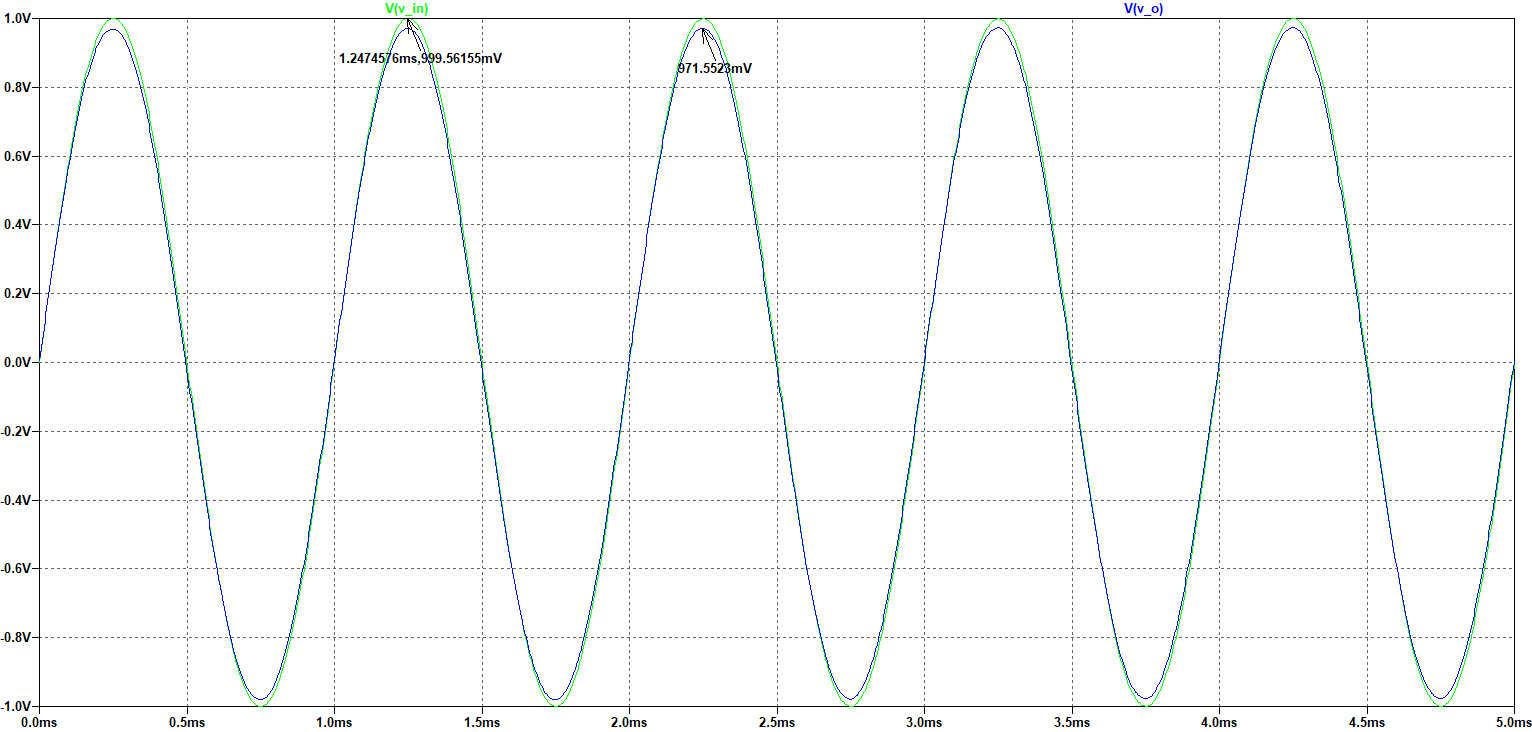
\includegraphics[width=\textwidth]{Imagenes/sim_voep.png}
          \caption{Simulación del voltaje de salida y entrada de la EP en tiempo}
          \label{fig:voep}
        \end{figure}

        Como Se puede apreciar en la imagen, se tiene en la simulación una ganancia de tensión casi 1.

        $$A_v=\dfrac{971.5523 m\volt}{999.5615 m\volt}= 0.971 \approx 1, $$

        siendo este valor el esperado.

        \textbf{Simulación para hallar la impedancia de entrada}

        Como se observa en la figura \ref{fig:zinep}, se tienen los valores pico de cada salida de voltaje de esta manera, haciendo uso de la ecuación \ref{eqn:zin}, tenemos lo siguiente:

        \begin{align*}
          Z_{in} & = V_i \dfrac{R_p}{V_g-V_i}      \\[0.2cm]
          Z_{in} & =\dfrac{646.86m(6k)}{1-646.86m} \\[0.2cm]
          Z_{in} & =10.99k\ohm                     \\[0.2cm]
        \end{align*}

        \begin{figure}[H]
          \centering
          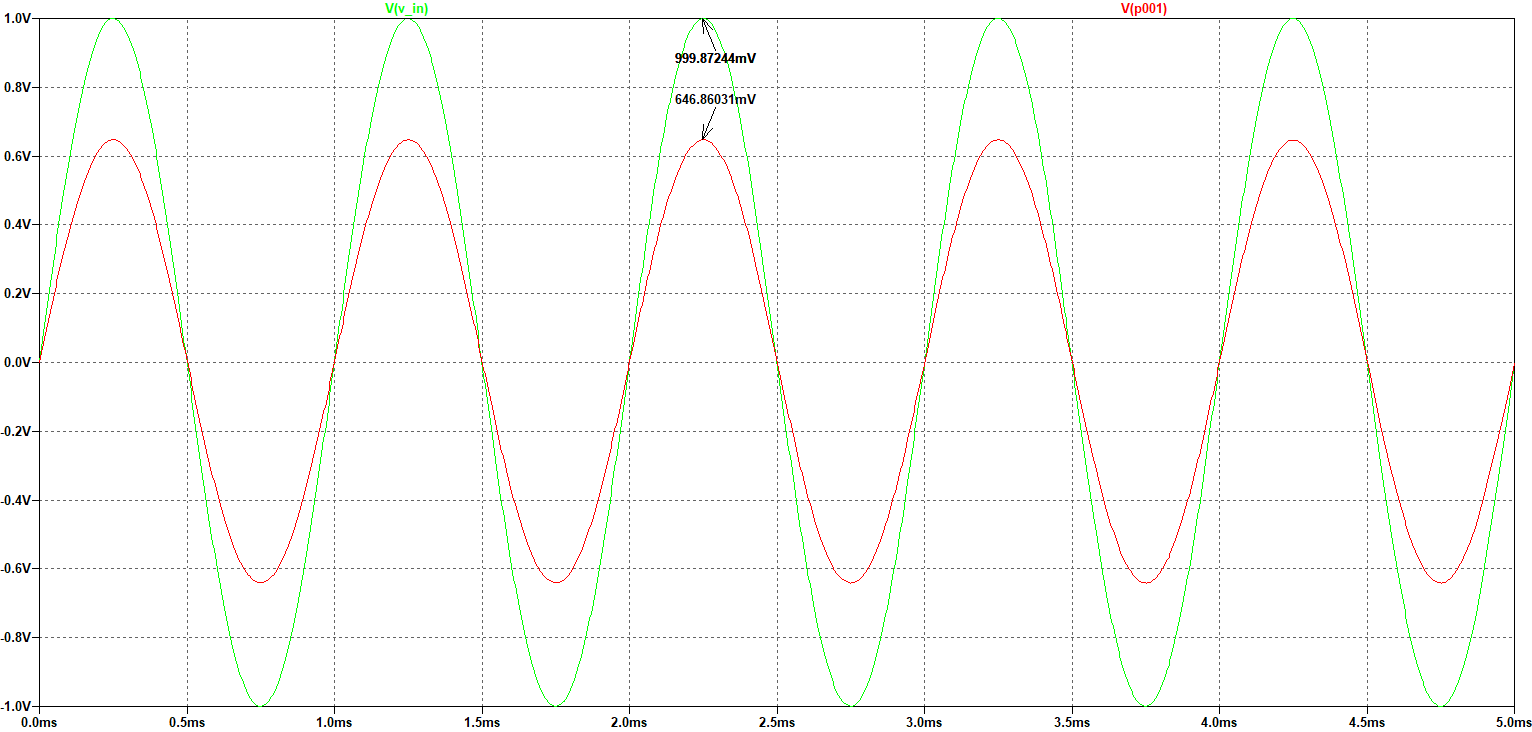
\includegraphics[width=\textwidth]{Imagenes/zinep.png}
          \caption{Simulación del voltaje de salida y entrada de la EP en tiempo para hallar la impedancia de entrada.}
          \label{fig:zinep}
        \end{figure}

        \textbf{Impedancia de salida}

        En este apartado, se va a establecer la impedancia de salida con la ecuación \ref{eqn:zo}, pero bajo las simulaciones realizadas previamente para la metodología adecuada del laboratorio.

        \begin{figure}[H]
          \centering
          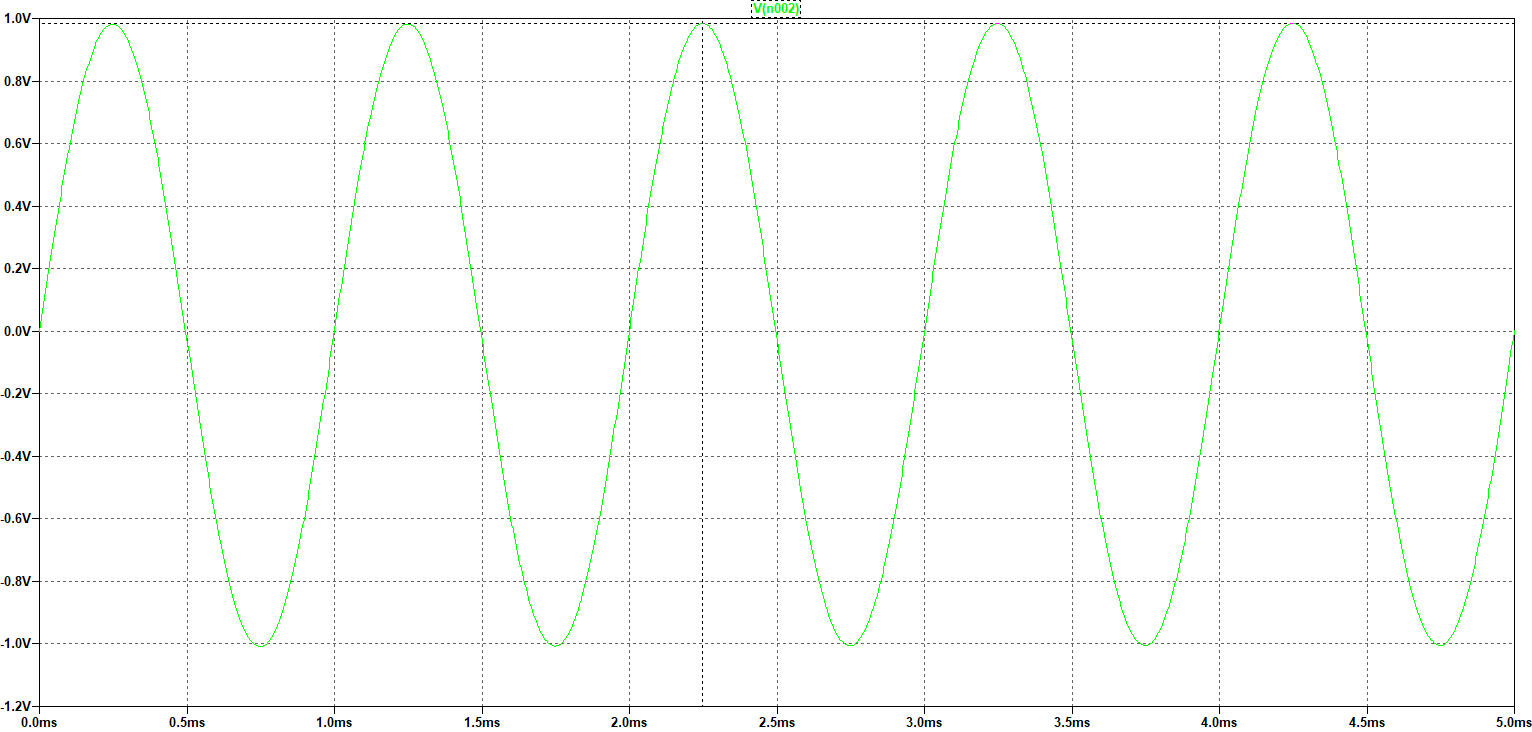
\includegraphics[width=\textwidth]{Imagenes/vo_sc_ep.png}
          \caption{Simulación del voltaje de salida sin carga de la ED en tiempo para hallar la impedancia de salida.}
          \label{fig:vo_sc_ep}
        \end{figure}

        En la figura \ref{fig:vo_sc_ep}, se visualiza el voltaje de salida sin carga, ahora se usara el valor de la simulación de la figura \ref{fig:vo_cc_ep}, y hallar la impedancia de salida.

        \begin{figure}[H]
          \centering
          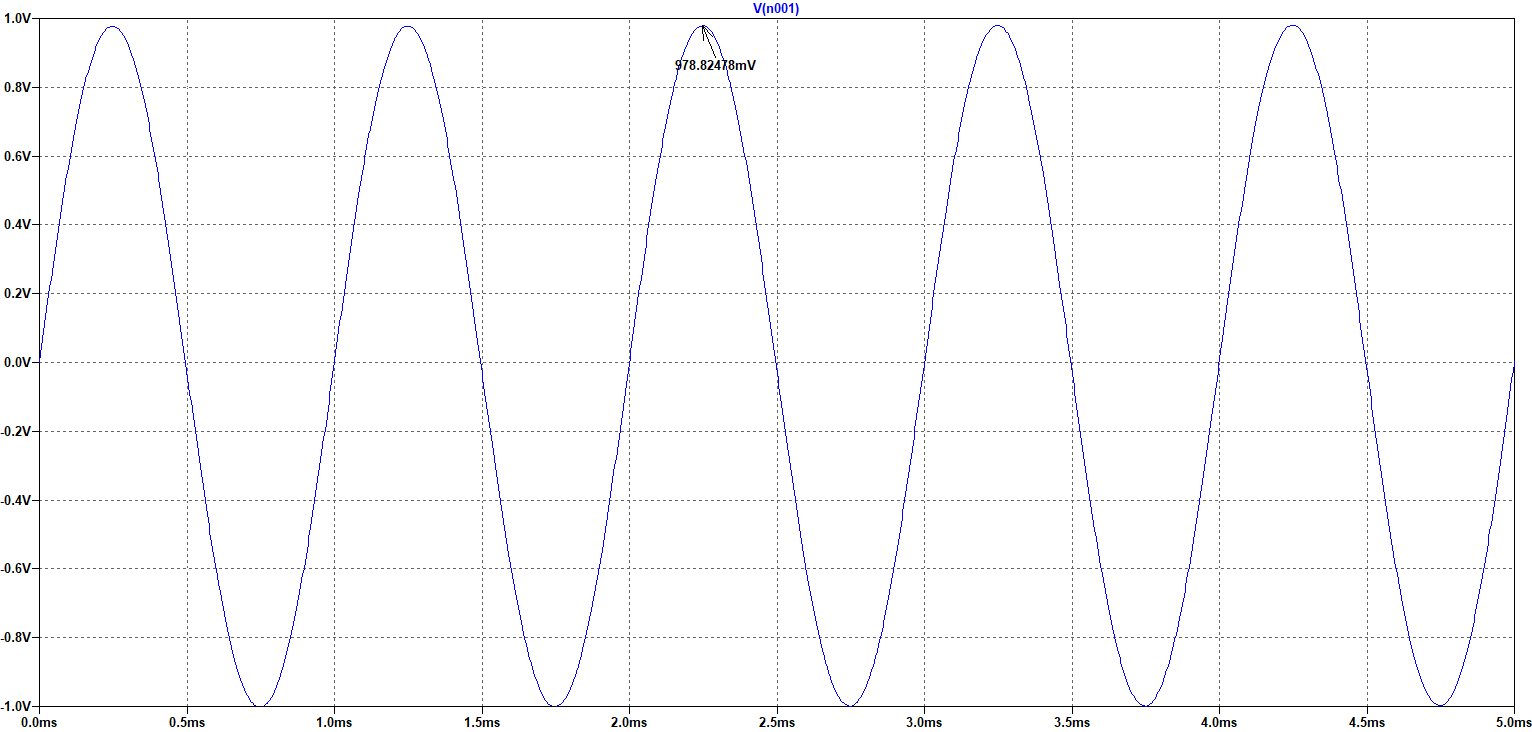
\includegraphics[width=\textwidth]{Imagenes/vo_cc_ep.png}
          \caption{Simulación del voltaje de salida con carga de la EP  en tiempo para hallar la impedancia de salida.}
          \label{fig:vo_cc_ep}
        \end{figure}

        \begin{align*}
          Z_{out} & = \dfrac{V_{osc}R_p - V_{occ}R_p}{V_{occ}} \\[0.2cm]
          Z_{out} & =\dfrac{(1.982-1.593)80}{1.593}            \\[0.2cm]
          Z_{out} & =19.535 \, \ohm                            \\[0.2cm]
        \end{align*}

        \begin{table}[H]
          \centering
          \begin{tabular}{|c|c|c|}
            \hline
            $\mathbf{A_v}$ & $\mathbf{Z_{in}[\ohm]}$ & $\mathbf{Z_{out} [\ohm]}$ \\ \hline
            0.971          & 10.99k                  & 19.535                    \\ \hline
          \end{tabular}
          \caption{Ganancia e impedancias simuladas de la Etapa de potencia}
          \label{tab:dinamico_ep_sim}
        \end{table}


\end{enumerate}

\subsection{Parte 2. Amplificador diferencial}

\begin{enumerate}
  \item \textbf{Identifique la etapa diferencial (ED) en el amplificador base (figura \ref{fig:amplificador_base}).}

        \begin{figure}[H]
          \centering
          \adjustbox{width = 5cm}{\begin{circuitikz}\draw
     \differential{dif}{out 3}
     (0,0) to [short,-o, label=$V_{o}$] ++(1,0) 
    (dif-in 1)  to[C,l=$C_{1}$,*-*] ++(-2,0) to[short,-o, label=$V_{in}$] ++(-0.5,0) (power-in 2) ++(0,10.75) node[vcc](VCC){$10\volt$} ++(0,-12.25) node[vee](VEE){$-10\volt$}
;\end{circuitikz}}
          \caption{Diagrama Esquemático de la etapa  diferencial}
          \label{fig:amplificador_diferencial}
        \end{figure}

        La etapa diferencial es la que se observa en la figura \ref{fig:amplificador_diferencial}, que se ve reflejada también en la figura \ref{fig:amplificador_base}, siendo la primera etapa del amplificador base.

  \item \textbf{Determinar los puntos de reposo de todos los transistores en la ED.}

        En esta etapa, los transistores $Q_1$ y $Q_2$ son iguales, debido a esto los puntos de operación de uno es igual para el otro.

        Hay que tener en cuenta que se tomará en cuenta lo dicho anteriormente con los transistores complementarios, debido a no estar bajo la misma oblea, ambos pueden tener pequeñas variaciones apreciables en su ganancia.

        \subsubsection{Análisis DC}

        Entonces, se tiene lo siguiente:

        \begin{align}
          Q_1=Q_2 \label{eqn:qeq} \\[0.2cm]
          I_{CQ_1}=I_{CQ_2}       \\[0.2cm]
          V_{CEQ_1}=V_{CEQ_2}
        \end{align}

        Tomando en cuenta esas consideraciones, la resistencia $R_5$ no sé tomará en cuenta en DC, ya que la caída de tensión entre sus puntos son iguales debido a la ecuación \ref{eqn:qeq}, por consiguiente, se trabajará con una sola configuración de los dos transistores.

        Simplificando el circuito de la polarización universal de la figura \ref{fig:universall}, obtenemos un $V_{th}$ y una $R_{th}$

        \begin{figure}[H]
          \centering
          \adjustbox{width = 3cm}{

\begin{circuitikz}\draw
     \universall{uni}{out 3}
     (0,0) to [short,-o, label=$V_{o}$] ++(1,0) 
    (dif-in 1)  to[C,l=$C_{1}$,*-*] ++(-2,0) to[short,-o, label=$V_{in}$] ++(-0.5,0) (power-in 2) ++(0,10.75) node[vcc](VCC){$10\volt$} ++(0,-12.25) node[vee](VEE){$-10\volt$}
;\end{circuitikz}}
          \caption{Polarización universal para el estudio del amplificador diferencial}
          \label{fig:universall}
        \end{figure}

        Se aplica divisor de tensión y superposición para hallar el  $V_{th}$:

        \begin{align*}
          V_{th} & = \dfrac{V_{CC}R_{2}}{R_1+R_2}+\dfrac{V_{EE}R_{1}}{R_1+R_2} \\[0.2cm]
          V_{th} & = \dfrac{10(100k)}{100k+100k}+\dfrac{-10(100k)}{100k+100k}  \\[0.2cm]
          V_{th} & = 5-5 = 0\volt                                              \\[0.2cm]
        \end{align*}

        Seguidamente se halla $R_{th}$
        \begin{align*}
          R_{th}=R_1||R_2=100k||100k=50k\ohm
        \end{align*}



        Aplicando la ecuación \ref{eqn:ic} y \ref{eqn:ie_ib}, se obtiene lo siguiente:
        $I_B$ se halla en un recorrido de lazo cerrado, de la base al emisor con el circuito simplificado
        \begin{align*}
          I_{CQ_1} & =\beta \dfrac{10-V_{BE_1}}{R_{th}+R_4(1+\beta)} \\[0.2cm]
          I_{CQ_1} & =\beta \dfrac{10-0.65}{50k+15k(151)}            \\[0.2cm]
          I_{CQ_1} & =605.832 \mu A                                  \\[0.2cm]
        \end{align*}

        Finalmente aplicando LVK por $V_{CE}$, se tiene


        \begin{align*}
          0         & =10-I_{CQ_1}(4.7k)-V_{CEQ_1}-\left(\dfrac{1+\beta}{\beta}\right)I_C(15k)+10 \\[0.2cm]
          V_{CEQ_1} & =20-I_{CQ_1}((4.7k)+\left(\dfrac{1+\beta}{\beta}\right)(15k))               \\[0.2cm]
          V_{CEQ_1} & = 8\volt                                                                    \\[0.2cm]
        \end{align*}

        \begin{table}[H]
          \centering
          \begin{tabular}{|c |c |c|}
            \hline %Lïnea horizontal
            \textbf{Transistor} & $\mathbf{I_{CQ}[\mu A]}$ & $\mathbf{V_{CEQ}[\volt]}$ \\
            \hline
            1                   & 605.832                  & 8                         \\
            \hline
            2                   & 605.832                  & 8                         \\
            \hline
          \end{tabular}
          \caption{Puntos de operación teóricos de la ED}
          \label{tab:ptos_ed}
        \end{table}

        \subsubsection{Análisis en AC}

  \item \textbf{Determine el modelo dinámico del amplificador diferencial a frecuencias medias superponiendo ambos modos. ( Ganancias diferencial y común, impedancias de entrada diferencial y común e impedancia de salida)}

        Como el anterior estudio del análisis en AC, acá se usaran las mismas ecuaciones y por consiguiente, se va a enfocar en colocar las ecuaciones y se darán los resultados de una manera directa para resumir cuentas.

        Se hallará $g_{m_1}$ y $r_{\pi_1}$, recordando que $Q_1=Q_2$, así tenemos que $g_{m_1}=g_{m_2}$ y $r_{\pi_1}=r_{\pi_2}$.

        \begin{align*}
          r_{\pi_1}= \beta \dfrac{V_T}{I_{CQ_5}} & =150 \dfrac{25.851 mA}{605.83 \mu A} \nonumber \\[0.2cm]
          r_{\pi_5}                              & =6.4k \ohm
        \end{align*}

        \begin{align*}
          g_{m_1} & =\dfrac{I_{CQ_5}}{V_T}=\dfrac{605.83 \mu A}{25.851 mA} \nonumber \\[0.2cm]
          g_{m_5} & =23.435m \mho
        \end{align*}


        \textbf{Ganancia de tensión}

        Para hallar la ganancia de tensión de un amplificador diferencial existen dos modos, denominados \textbf{Modo diferencial y Modo Común}, y cada uno de ellos posee una configuración distinta, sin embargo son sencillas de comprender topológicamente.

        En este apartado usaremos las ecuaciones \ref{eqn:ac} y  \ref{eqn:ad}.

        \begin{itemize}
          \item \textbf{Modo diferencial}
                En este punto, la topología a visualizar en modo diferencias es la que se ve en la figura \ref{fig:amplificador_diferencial}, siendo las entradas las bases de los transistores $Q_1$ y $Q_2$, sin embargo, acá solo se tiene una entrada que es por la base de $Q_1$, ya conociendo esto se procede a los cálculos de ganancia de tensión. (Aplica de igual manera para la impedancia en modo diferencial)


                \textbf{Nota:} en modo diferencial tomamos en cuenta la resistencia $R_5$ debido a la configuración que se ve en la figura \ref{fig:amplificador_diferencial}, el recorrido de su corriente es por $R_5$, ya que $R_4$ y $R_7$ son mucho mas grande que $R_5$, además que al no estar en modo común, pasa una corriente distinta por ambas entradas, de esta manera, tiene la posibilidad de solo tomar en cuenta $R_5$ y despreciar la corriente que pasa por $R_4$ y $R_7$. Por el contrario, en modo Común, al tener la misma entrada y ésta dividirse en dos, entra la misma corriente, debido a eso las corrientes que pasa por $R_5$ se anulan, permitiendo que no se desprecie la corriente que pasa por $R_4$ y $R_7$. Por lo tanto, este análisis facilita la obtención de sus ganancias e impedancias de una manera más óptima.
                \begin{align*}
                  A_d & = -\dfrac{(g_{m_1}r_{\pi_1})R_3}{r_{\pi_1}+(g_{m_1}r_{\pi_1}+1)\left(R_{5}+\dfrac{r_{\pi_2}}{(g_{m_2}r_{\pi_2}+1)}\right) } \\[0.2cm]
                  A_d & = -2.95 \approx 3                                                                                                           \\[0.2cm]
                \end{align*}
          \item \textbf{Modo común}
                La topología de esta configuración es haciendo las entradas una sola, es decir hacemos un corto circuito entre las bases de $Q_1$ y $Q_2$, logrando tener un modo común con la entrada de la señal de la fuente, por esa razón su nombre.
                \begin{align*}
                  A_c & =- \dfrac{(g_{m_1}r_{\pi_1})R_3}{r_{\pi_1}+(g_{m_1}r_{\pi_1}+1)R_{4}} \\[0.2cm]
                  A_c & = -0.31                                                               \\[0.2cm]
                \end{align*}
        \end{itemize}
        \newpage
        \textbf{Modelo de Impedancias}

        \begin{itemize}
          \item \textbf{Impedancia en modo diferencial}
                Acá manejamos la misma topología que en ganancia, al igual que su recorrido de corriente.
                \begin{align}
                  Z_d   & = R_{1}||R_{2}||(r_{\pi_1}+ (g_{m_1}r_{\pi_1}+1)
                  \left(R_{5}+\dfrac{r_{\pi_2}}{(g_{m_2}r_{\pi_2}+1)}\right)) \nonumber \\[0.2cm]
                  Z_d   & = R_{1}||R_{2}||(2r_{\pi_1}+
                  R_{5}(g_{m_1}r_{\pi_1}+1))\nonumber                                   \\[0.2cm]
                  Z_{d} & = 41.36k\ohm \label{eqn:zd}
                \end{align}

          \item \textbf{Impedancia en modo común}
                \begin{align*}
                  Z_c & =R_1||R_2||r_{\pi_1}+(g_{m_1}r_{\pi_1}+1)R_{4} \\[0.2cm]
                  Z_c & =48.82k \ohm                                   \\[0.2cm]
                \end{align*}

          \item \textbf{Impedancia de Salida}
                \begin{align*}
                  Z_{out} & =R_3       \\[0.2cm]
                  Z_{out} & =4.7k \ohm \\[0.2cm]
                \end{align*}


          \item \textbf{Nota:} Una acotación importante es que en este apartado se da lo que conocemos como \textbf{CMRR}, como se observa en la ecuación \ref{eqn:cmrr}, si se analiza, se tiene que si $\mathbf{A_d}$ aumenta se va a obtener una mayor ganancia evitando el $\mathbf{CMRR}$ siendo este valido cuando $\mathbf{CMRR=\rho \geq 100db}$, para que esto ocurra de una mejor manera $\mathbf{A_c}$ debería dar muy bajo, para poder su efecto de rechazo alto.

                Para eso realizamos este calculo, para poder ver si existe una buena ganancia. Sin embargo, de no tener una diferencia de potencial en las dos entradas AC no existirá una ganancia.
        \end{itemize}

        \begin{table}[H]
          \centering
          \begin{tabular}{|c|c|c|c|c|c|}
            \hline
            $\mathbf{A_v}$ & $\mathbf{A_C}$ & $\mathbf{Z_{d}[\ohm]}$ & $\mathbf{Z_{c}[\ohm]}$ & $\mathbf{Z_{out} [\ohm]}$ & $\mathbf{\rho [dB]}$ \\ \hline
            -2.95          & -0.31          & 41.36 k                & 48.85k                 & 4.7k                      & 19.57                \\ \hline
          \end{tabular}
          \caption{Ganancia e impedancias teóricas de la Etapa diferencial}
          \label{tab:dinamico_ed}
        \end{table}

        \subsubsection{Simulación}

  \item Realice la simulación de la etapa con el fin de verificar los cálculos de los puntos de operación y el
        modelo dinámico.

        \begin{table}[H]
          \centering
          \begin{tabular}{|c|c|c|}
            \hline
            \textbf{Tag} & \textbf{Puntos de operación} & \textbf{Unidad} \\
            \hline
            V(v\_ce2)    & 8.850259                     & voltage         \\\hline
            V(v\_ce1)    & 7.207804                     & voltage         \\\hline
            Ic(Q1)       & 7.57E-04                     & device\_current \\\hline
            Ic(Q2)       & 4.53E-04                     & device\_current \\
            \hline
          \end{tabular}
          \caption{Simulación de los puntos de operación de la ED}
          \label{tab:ptos_ope_ed}
        \end{table}

        Se aprecian unas diferencias, se calcularan los errores relativos porcentuales, estas diferencias se deben a que son el mismo encapsulado y poseen las mismas características y especificaciones, pero ambos están creado bajos distintas obleas de silicio.

        \begin{itemize}
          \item $\mathbf{V_{CE_1}}$
                \begin{align*}
                  V_{CE_1}=7.21\volt
                  E_r & =\dfrac{|8-7.21|}{8}\cdot 100 \\[0.2cm]
                  E_r & =9.875\%
                \end{align*}

          \item $\mathbf{V_{CE_2}}$
                \begin{align*}
                  V_{CE_2}=8.85\volt
                  E_r & =\dfrac{|8-8.85|}{8}\cdot 100 \\[0.2cm]
                  E_r & =3.125\%
                \end{align*}

          \item $\mathbf{I_{CQ_1}}$
                \begin{align*}
                  I_{CQ_1} & =757 \mu A                                    \\[0.2cm]
                  E_r      & =\dfrac{|605.832\mu-757\mu|}{425\mu}\cdot 100 \\[0.2cm]
                  E_r      & =24.34\%
                \end{align*}
          \item $\mathbf{I_{CQ_2}}$
                \begin{align*}
                  I_{CQ_2} & =453 \mu A                                    \\[0.2cm]
                  E_r      & =\dfrac{|605.832\mu-453\mu|}{425\mu}\cdot 100 \\[0.2cm]
                  E_r      & =25.23\%
                \end{align*}
        \end{itemize}


        Como se puede apreciar, cada uno de los errores relativos porcentuales no son despreciables, pero validos para los cálculos teóricos realizados, se aproximan bastante a los posibles. Más adelante sabremos si nos acercamos bastante a los valores experimentales o reales.
        \newpage
        \textbf{Simulación de ganancia en tiempo}

        \begin{figure}[H]
          \centering
          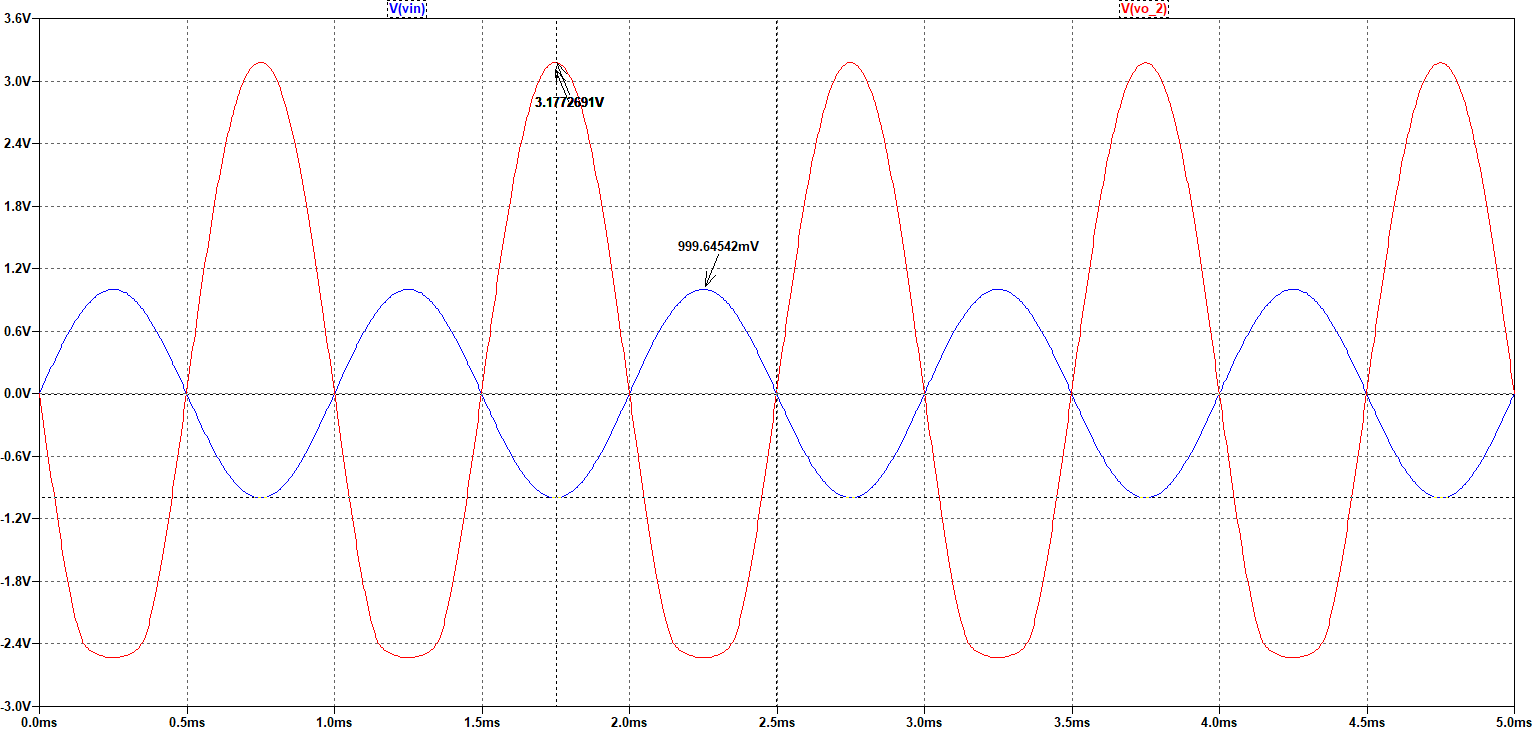
\includegraphics[width=\textwidth]{Imagenes/sim_voed.png}
          \caption{Simulación del voltaje de salida y entrada de la ED en tiempo}
          \label{fig:voed}
        \end{figure}

        Como Se puede apreciar en la imagen, se tiene en la simulación una ganancia de tensión de:

        $$A_v=\dfrac{3.1772691\volt}{0.99964542\volt}= 3.178, $$

        siendo este valor el esperado.

        \begin{itemize}
          \item \textbf{Nota: } Se calculo la ganancia e indico un valor negativo, esto es debido al desfase que ocurre que es de 180°, y que posee una ganancia donde entra por base y sale por colector, podría verse como una configuración de emisor-Común estando dos en paralelo.

                Por consiguiente, la figura \ref{fig:voed} se pueden apreciar el desfase y su ganancia. Comportándose en la zona lineal por la polarización universal.
        \end{itemize}

        \textbf{Simulación para hallar la impedancia en modo diferencial}

        Como se observa en la figura \ref{fig:zded}, se tienen los valores pico de cada salida de voltaje de esta manera, haciendo uso de la ecuación \ref{eqn:zin}, tenemos lo siguiente:

        \begin{align*}
          Z_{d} & = V_i \dfrac{R_p}{V_g-V_i}           \\[0.2cm]
          Z_{d} & =\dfrac{520.066m(41.5k)}{1-520.066m} \\[0.2cm]
          Z_{d} & =\dfrac{520.066m(41.5k)}{1-520.066m} \\[0.2cm]
          Z_{d} & =44.97k\ohm                          \\[0.2cm]
        \end{align*}

        \begin{figure}[H]
          \centering
          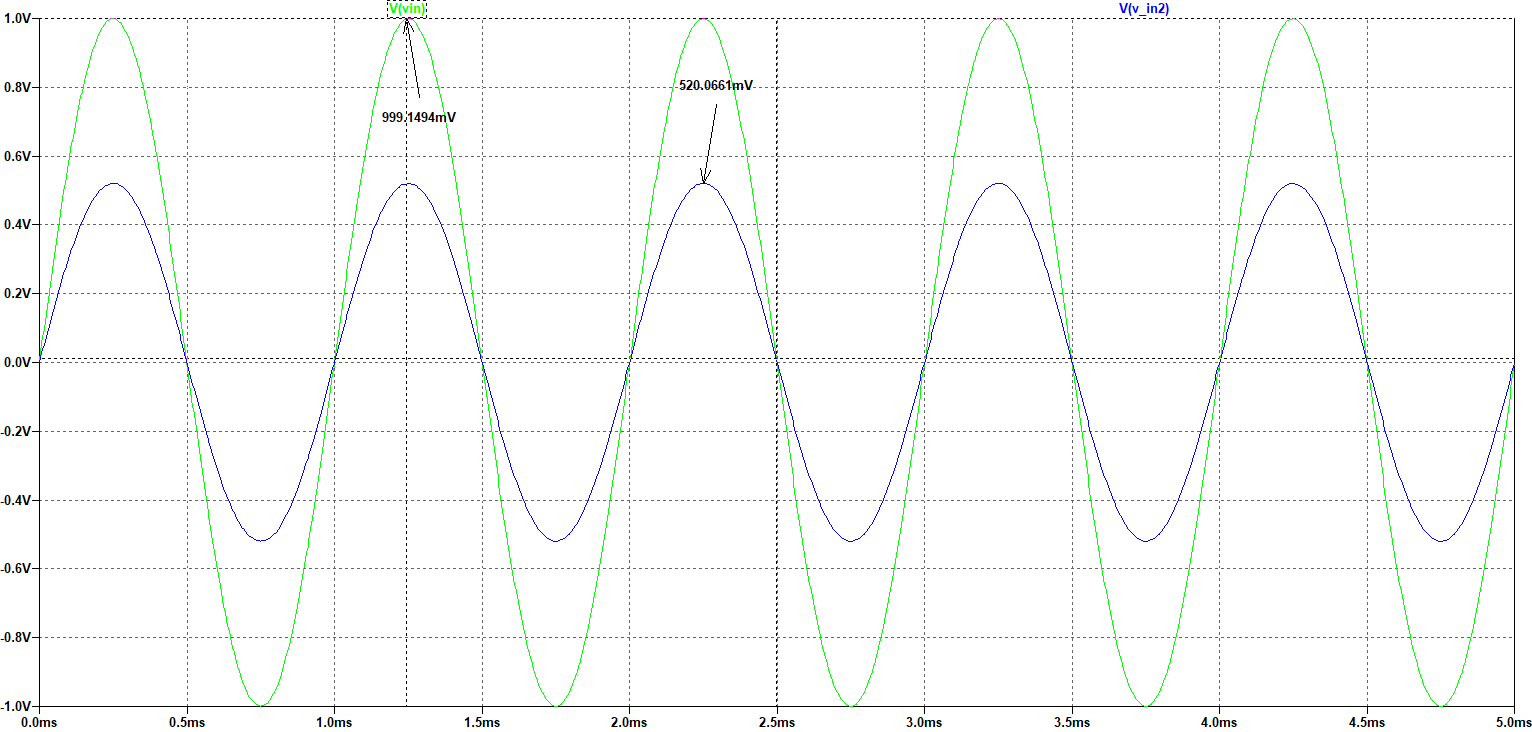
\includegraphics[width=\textwidth]{Imagenes/zd_ed.png}
          \caption{Simulación del voltaje de salida y entrada de la ED en tiempo para hallar la impedancia en modo diferencial.}
          \label{fig:zded}
        \end{figure}

        \textbf{Simulación para hallar la impedancia en modo común}

        Como se observa en la figura \ref{fig:zced}, se tienen los valores pico de cada salida de voltaje de esta manera, haciendo uso de la ecuación \ref{eqn:zc}, tenemos lo siguiente:

        \begin{align*}
          Z_{c}            & = 2V_i \dfrac{R_p}{V_g-V_i}         \\[0.2cm]
          Z_{c}            & =2\dfrac{520.066m(50k)}{1-520.066m} \\[0.2cm]
          Z_{c}            & =2\dfrac{520.066m(50k)}{1-520.066m} \\[0.2cm]
          Z_{c}            & =108.36k\ohm                        \\[0.2cm]
          \dfrac{Z_{c}}{2} & =54.18k\ohm                         \\[0.2cm]
        \end{align*}

        \begin{figure}[H]
          \centering
          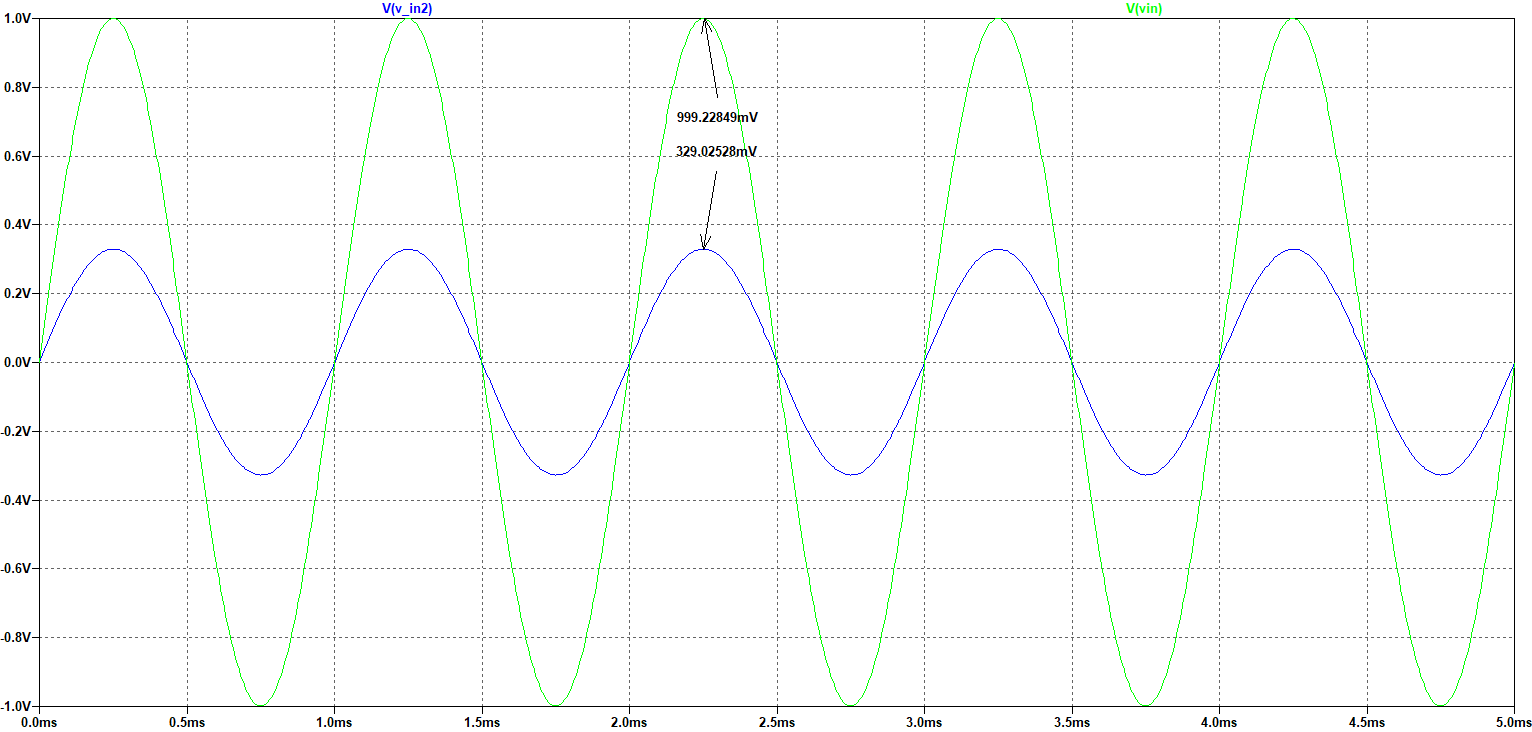
\includegraphics[width=\textwidth]{Imagenes/zc_ed.png}
          \caption{Simulación del voltaje de salida y entrada de la ED en tiempo para hallar la impedancia en modo común.}
          \label{fig:zced}
        \end{figure}

        \textbf{Impedancia de salida}

        En este apartado, se va a establecer la impedancia de salida con la ecuación \ref{eqn:zo}, pero bajo las simulaciones realizadas previamente para la metodología adecuada del laboratorio.

        \begin{figure}[H]
          \centering
          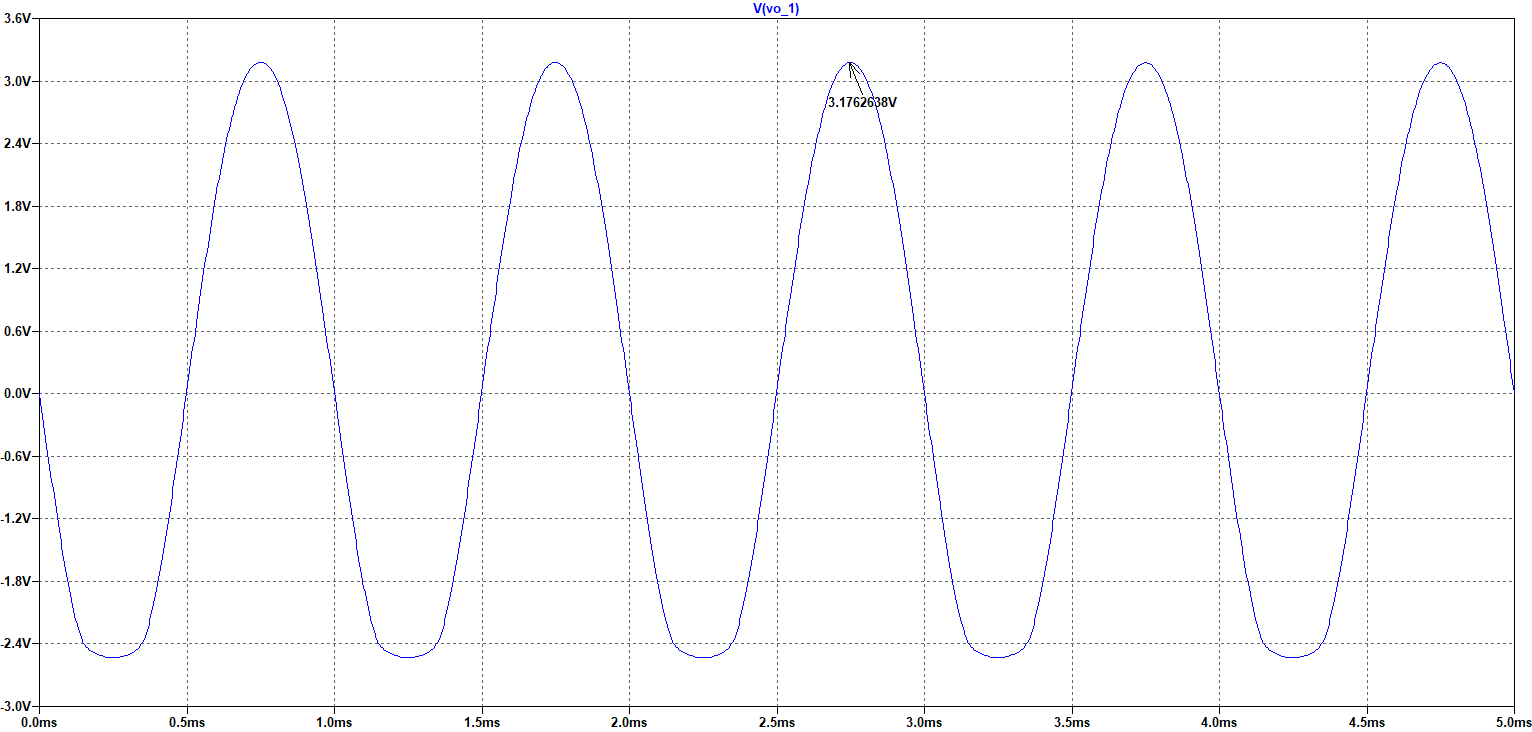
\includegraphics[width=\textwidth]{Imagenes/vosc.png}
          \caption{Simulación del voltaje de salida sin carga de la ED en tiempo para hallar la impedancia de salida.}
          \label{fig:vo_sc_ed}
        \end{figure}

        En la figura \ref{fig:vo_sc_ed}, se visualiza el voltaje de salida sin carga, ahora se usara el valor de la simulación de la figura \ref{fig:vo_cc_ed}, y hallar la impedancia de salida.

        \begin{figure}[H]
          \centering
          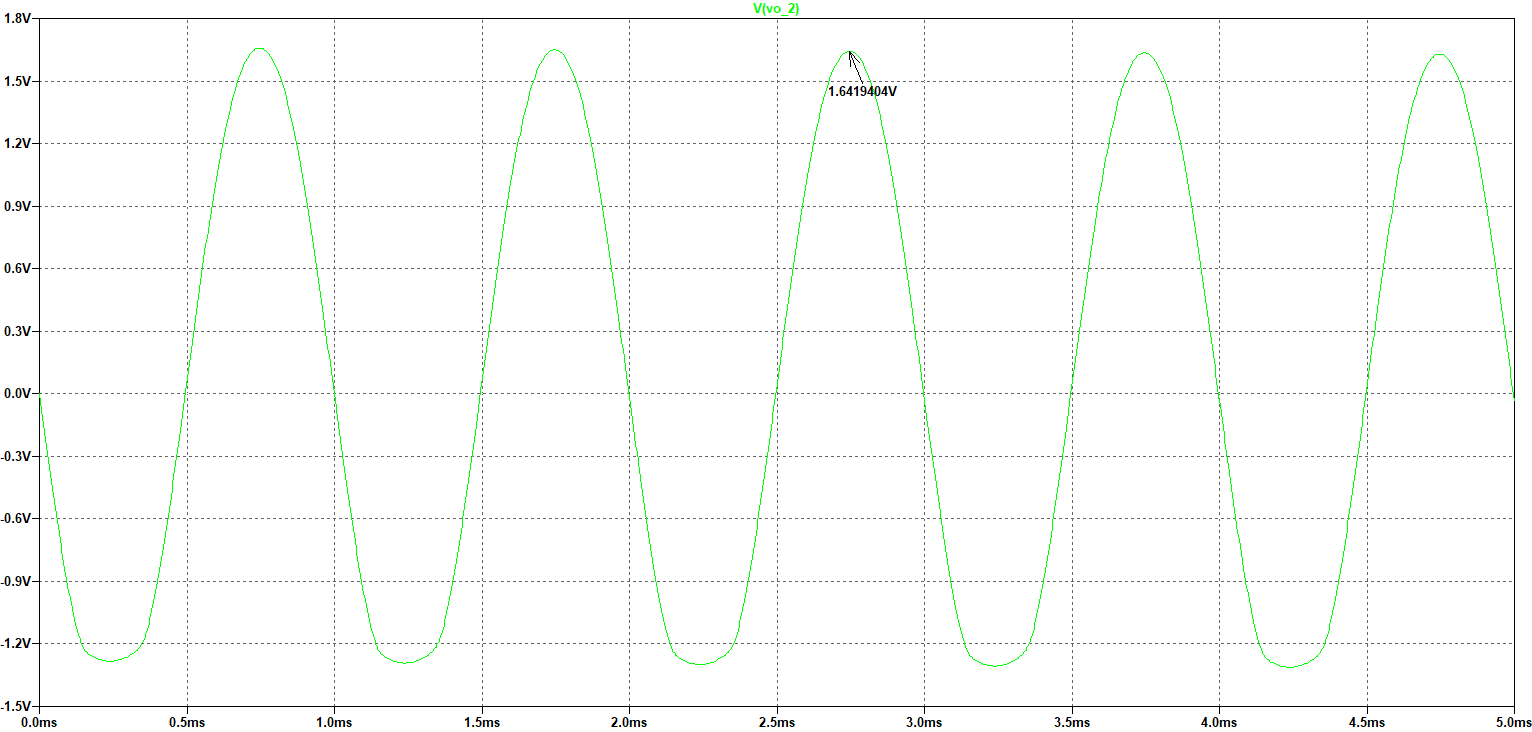
\includegraphics[width=\textwidth]{Imagenes/vocc.png}
          \caption{Simulación del voltaje de salida con carga de la ED en tiempo para hallar la impedancia de salida.}
          \label{fig:vo_cc_ed}
        \end{figure}

        \begin{align*}
          Z_o     & = \dfrac{V_{osc}R_p - V_{occ}R_p}{V_{occ}} \\[0.2cm]
          Z_{out} & =\dfrac{(3.17626-1.64194)5k}{1.64194}      \\[0.2cm]
          Z_{out} & =4.67k                                     \\[0.2cm]
        \end{align*}

        \begin{table}[H]
          \centering
          \begin{tabular}{|c|c|c|c|}
            \hline
            $\mathbf{A_v}$ & $\mathbf{Z_{d}[\ohm]}$ & $\mathbf{Z_{c}[\ohm]}$ & $\mathbf{Z_{out} [\ohm]}$ \\ \hline
            -3.178         & 44.97k                 & 54.18k                 & 4.67k                     \\ \hline
          \end{tabular}
          \caption{Ganancia e impedancias simuladas de la Etapa diferencial}
          \label{tab:dinamico_ed_sim}
        \end{table}

\end{enumerate}

\subsection{Parte 3. Amplificador multietapas}

\begin{enumerate}
  \item \textbf{Para cada etapa por separado del amplificador base (figura \ref{fig:amplificador_base}) determine: Punto de operación de los elementos activos y modelo dinámico de las etapas amplificadoras. Utilice como carga $R_L$ la indicada en el anexo ($R_L=2.2k\ohm$).}

        Los puntos operacionales de la etapa de potencia están reflejados en la tabla \ref{tab:ptos_ep} y los de la etapa diferencial en la tabla \ref{tab:ptos_ed}.

        Los puntos del modelo dinámico de la etapa de potencia se hallan en la tabla \ref{tab:dinamico_ep} y la etapa diferencial en la tabla \ref{tab:dinamico_ed}.

        \subsubsection{Análisis DC}
        Se va a calcular los puntos de operación y modelo dinámico de la etapa impulsora o driver. Se identifica a la etapa impulsora en el amplificador base directamente en la figura \ref{fig:driver}

        \begin{figure}[H]
          \centering
          \adjustbox{width = 3cm}{\begin{circuitikz}\draw
    (0,0)\driver{driv}{out 3} to[C,l=$C_{7}$,*-*]++(3,0) 
;\end{circuitikz}}
          \caption{Diagrama esquemática de la etapa impulsora}
          \label{fig:driver}
        \end{figure}

        En la figura \ref{fig:driver} se tiene el capacitor $C_7$ como capacitor de desacople, $C_6$ es un capacitor denominado de \textbf{bypass}, este nos permite que cuando este en su punto de operación permite una mayor ganancia debido a que tenemos la resistencia $R_{11}$  que ayuda a su punto de operación, pero en AC, no se toma en cuenta gracias al condensador. Por otro lado, permite que al ver la impedancia de $Z_{CCQ_3}$, solo observará $r_0$, a consecuencia de el capacitor de bypass, por el corto generado a frecuencias medias y en AC.

        El condensador $C_4$ se comporta como un abierto al igual que todos las demás capacitores, a diferencia es que los demás se cortocircuitan en frecuencias medias (en AC), este solo se cortocircuita en frecuencias altas, esto se identifica por su valor de capacitancia y que se encuentra entre Base y Colector, manejando el modelo expandido de pi, tomando en cuentas las perdidas en alta frecuencia.

        Al igual que con la etapa de diferencial, se aplica divisor de tensión y superposición para hallar el $V_{th}$.

        Esto es debido a que se simplifica el circuito realizando un circuito equivalente visto desde la base hacia la entrada.

        \begin{align*}
          V_{th} & = \dfrac{V_{CC}R_{10}}{R_{10}+R_{15}}+\dfrac{V_{EE}R_{15}}{R_{10}+R_{15}} \\[0.2cm]
          V_{th} & = \dfrac{10(220k)}{220k+33k}+\dfrac{-10(33k)}{220k+33k}                   \\[0.2cm]
          V_{th} & = 7.4 \volt                                                               \\[0.2cm]
        \end{align*}

        Seguidamente se halla $R_{th}$
        \begin{align*}
          R_{th}=R_{15}||R_{10}=33k||220k=28.7k\ohm
        \end{align*}

        Aplicando LVK, al circuito equivalente de thevenin de la figura \ref{fig:driver}, se halla $I_{CQ_3}$, haremos uso de la ecuación \ref{eqn:ib}

        \begin{align*}
          0        & =10-I_CR_{11}-V_{EB}-I_{B}R_{th}-V_{th}                 \\[0.2cm]
          I_{CQ_3} & =\dfrac{10-V_{BE}-V_{th}}{R_{11}+\dfrac{R_{th}}{\beta}} \\[0.2cm]
          I_{CQ_3} & =\dfrac{10-0.65-7.4}{680+\dfrac{28.7k}{150}}            \\[0.2cm]
          I_{CQ_3} & =2.24mA                                                 \\[0.2cm]
        \end{align*}

        Finalmente, se halla $V_{CEQ_3}$, aplicando LVK por el transistor $Q_3$

        \begin{align*}
          0         & =10-I_{E}(R_{11})-V_{CEQ_3}-I_C(R_{16})+10 \\[0.2cm]
          V_{CEQ_3} & =20-I_{E}(R_{11})-I_C(R_{16})              \\[0.2cm]
          V_{CEQ_3} & = 3.2346\volt                              \\[0.2cm]
        \end{align*}

        \begin{table}[H]
          \centering
          \begin{tabular}{|c |c |c|}
            \hline %Lïnea horizontal
            \textbf{Transistor} & $\mathbf{I_{CQ}[ A]}$ & $\mathbf{V_{CEQ}[\volt]}$ \\
            \hline
            3                   & 2.24m                 & 3.2346                    \\
            \hline
          \end{tabular}
          \caption{Puntos de operación teóricos de la etapa impulsora}
          \label{tab:ptos_ei}
        \end{table}

        \subsubsection{Análisis en AC}
        Se hallará $g_{m_3}$, $r_{\pi_3}$ y $r_0$, recordar que se hace uso de las ecuaciones \ref{eqn:gm}, \ref{eqn:rpi} y \ref{eqn:ro}.

        \begin{align*}
          r_{\pi_3}= \beta \dfrac{V_T}{I_{CQ_3}} & =150 \dfrac{25.851 mA}{2.24 mA} \nonumber \\[0.2cm]
          r_{\pi_3}                              & =1.732k \ohm
        \end{align*}

        \begin{align*}
          g_{m_3} & =\dfrac{I_{CQ_3}}{V_T}=\dfrac{2.24m A}{25.851 mA} \nonumber \\[0.2cm]
          g_{m_3} & =86.65m \mho
        \end{align*}

        En este caso, $r_0$ es distinto de infinito, debido a que este transistor $Q_3$, posee un capacitor que se tomará en cuenta en altas frecuencias, aplicando el teorema de Miller, por el modelo expandido de pi. Siendo un capacitor asociado a la juntura del transistor.

        \begin{gather}
          r_0=\dfrac{V_A}{I_C}=\dfrac{150}{2.24m} \nonumber \\[0.2cm]
          r_0=67.024 \, K\ohm
        \end{gather}

        \textbf{Ganancia de tensión}

        \begin{align*}
          A_v & =- \dfrac{g_{m_3}r_{\pi_3}R_{16}}{r_{\pi_3}} \\[0.2cm]
          A_v & =- \dfrac{150(6.8k)}{1.732k}                 \\[0.2cm]
          A_v & =- -588.91                                   \\[0.2cm]
        \end{align*}

        Lo que se obtiene como resultado, da una mayor relación como su nombre lo indica, \"impulsora\", en efecto se tiene una ganancia bastante grande, que permite impulsar la señal de la etapa anterior, siendo la de la etapa diferencial.

        \textbf{Impedancia de entrada}

        \begin{align*}
          Z_{in} & = R_{15}||R_{10}||r_{\pi_3} \\[0.2cm]
          Z_{in} & = 1.633k\ohm
        \end{align*}

        \textbf{Impedancia de salida}

        \begin{align*}
          Z_{out} & = R_{16}    \\[0.2cm]
          Z_{out} & = 6.8k \ohm
        \end{align*}

        \begin{table}[H]
          \centering
          \begin{tabular}{|c|c|c|}
            \hline
            $\mathbf{A_v}$ & $\mathbf{Z_{in}[\ohm]}$ & $\mathbf{Z_{out} [\ohm]}$ \\\hline
            -588.91        & 1.633k                  & 6.8k                      \\\hline
          \end{tabular}
          \caption{Ganancia e impedancias teóricas de la Etapa impulsora}
          \label{tab:dinamico_ei}
        \end{table}

  \item \textbf{Acoplando todas las etapas del amplificador base, determine: Punto de operación de los elementos activos
          y modelo dinámico del amplificador completo.}

        Debido a los condensadores de acople y desacople ($C_1$, $C_2$, $C_3$, $C_5$, $C_6$ y $C_7$ ), los puntos de operación se mantienen igual para cada una de las etapas, como se indica anteriormente sus valores se hallan en la tabla \ref{tab:ptos_ed}, \ref{tab:ptos_ep} y \ref{tab:ptos_ei}

        Lo que si cambia es el estudio en su modelo dinámico, debido a la ecuación \ref{eqn:capacitores}, donde cada uno de los capacitores de acople y desacople se comportan como un corto, exceptuando el capacitor $C_4$, donde se realizará un estudio mas detallado en los próximos apartados.


        En este análisis como se están acoplando las distintas etapas, para hallar la Ganancia total, se aplicará la ecuación \ref{eqn:avt}.

        Aunque se representara en la \textbf{tabla \ref{tab:gm_rpi} }
        , donde podemos encontrar de manera inmediata cada uno de los valores de $g_{m}$, $r_\pi$ y $r_o$.

        \begin{table}[H]
          \centering
          \begin{tabular}{|c|c|c|c|}
            \hline
            \textbf{Transistores} & $\mathbf{g_m [\si{\mho}]}$ & $\mathbf{r_\pi [\si{\ohm}]}$ & $\mathbf{r_o [\ohm]}$ \\
            \hline
            1                     & 23.435m                    & 6.4k                         & $\infty$              \\\hline
            2                     & 23.435m                    & 6.4k                         & $\infty$              \\\hline
            3                     & 86.65m                     & 1.732k                       & 67.024k               \\\hline
            5                     & 16.44m                     & 9.124k                       & $\infty$              \\\hline
            6                     & 16.44m                     & 9.124k                       & $\infty$              \\
            \hline
          \end{tabular}
          \caption{Valores de $g_{m}$, $r_\pi$ y $r_o$ del amplificador multietapas}
          \label{tab:gm_rpi}
        \end{table}

        Se tiene en cuenta la tabla ahora se busca la ganancia.

        \textbf{Ganancia de tensión de un amplificador multietapas}

        \begin{itemize}
          \item \textbf{Ganancia en modo Diferencial}

                \begin{align*}
                  A_v          & =A_dA_2A_3                                                                                                                                           \\[1cm]
                  A_d          & =-\dfrac{(g_{m_1}r_{\pi_1})(R_{3}||R_{15}||R_{10}||r_{\pi_3})}{r_{\pi_1}+(g_{m_1}r_{\pi_1}+1)\left(R_5+\dfrac{r_{\pi_2}}{g_{m_2}r_{\pi_2}+1}\right)} \\[0.2cm]
                  A_d          & =-0.755                                                                                                                                              \\[1cm]
                  A_2          & =-\dfrac{(g_{m_3}r_{\pi_3})(R_{16}||R_{17}||R_{12}||(r_{\pi_5}+(g_{m_5}r_{\pi_5}+1)(R_{13}+R_L)))}{r_{\pi_3}}                                        \\[0.2cm]
                  A_2          & =-363.128                                                                                                                                            \\[1cm]
                  A_3          & =\dfrac{(g_{m_5}r_{\pi_5}+1)(R_{13}+R_L)}{r_{\pi_5}+(g_{m_5}r_{\pi_5}+1)(R_{13}+R_L)}\left(\dfrac{R_L}{R_{13}+R_L}\right)                            \\[0.2cm]
                  A_3          & =0.969                                                                                                                                               \\[1cm]
                  A_v          & =-0.755(-363.128)0.969                                                                                                                               \\[0.2cm]
                  \mathbf{A_v} & =\mathbf{265.659} = 20log(265.659)=48.487 db                                                                                                         \\[0.2cm]
                \end{align*}

          \item \textbf{Ganancia en modo Común}

                En este caso, la ganancia de $A_2$ y $A_3$ se mantienen iguales y solo cambia la de la etapa diferencial acoplada con las demás etapas.

                \begin{align*}
                  A_{vc}          & =A_cA_2A_3                                                                                        \\[1cm]
                  A_c             & =-\dfrac{(g_{m_1}r_{\pi_1})(R_{3}||R_{15}||R_{10}||r_{\pi_3})}{r_{\pi_1}+(g_{m_1}r_{\pi_1}+1)R_4} \\[0.2cm]
                  A_c             & =-0.0795                                                                                          \\[1cm]
                  A_2             & =-363.128                                                                                         \\[1cm]
                  A_3             & =0.969                                                                                            \\[1cm]
                  A_{vc}          & =-0.0795 (-363.128 )0.969                                                                         \\[0.2cm]
                  \mathbf{A_{vc}} & =\mathbf{27.973}                                                                                  \\[0.2cm]
                \end{align*}

        \end{itemize}
        \textbf{Impedancia de entrada modo diferencial}

        Se puede observar en el circuito de la figura \ref{fig:amplificador_base}, que la impedancia de entrada es el mismo que la impedancia de entrada en modo diferencial de la etapa diferencial. Por lo tanto, haciendo uso del valor de la ecuación \ref{eqn:zd}, se tiene:
        $$Z_{in}=Z_d=41.36k\si{\ohm}$$



        \textbf{Impedancia de entrada modo común}

        Se puede observar en el circuito de la figura \ref{fig:amplificador_base}, que la impedancia de entrada es el mismo que la impedancia de entrada en modo común de la etapa diferencial. Por lo tanto, haciendo uso del valor de la ecuación \ref{eqn:zc}, se tiene y también sale reflejado en la tabla \ref{tab:dinamico_ed}:
        $$Z_{in}=Z_c=48.82k\si{\ohm}$$

        \textbf{Impedancia de salida}

        Recordar que ayuda mucho observar desde donde estas viendo el circuito y de esa manera empezar allí el recorrido de la corriente para dar el resultado adecuado.

        \begin{align*}
          Z_{out} & =\left(\dfrac{R_L}{R_{13}+R_L}\right)[R_{13}+R_L + \dfrac{r_{\pi_5}]||R_{16}||R_{17}||R_{12}}{g_{m_5}r_{\pi_5}+1} \\[0.2cm]
          Z_{out} & = 27.49 \si{\ohm}
        \end{align*}

        \begin{table}[H]
          \centering
          \begin{tabular}{|c|c|c|c|c|}
            \hline
            $\mathbf{A_v}$ & $\mathbf{A_{vc}}$ & $\mathbf{Z_{d}[\ohm]}$ & $\mathbf{Z_{c}[\ohm]}$ & $\mathbf{Z_{out} [\ohm]}$ \\\hline
            265.659        & 27.91             & 41.36k                 & 48.82k                 & 27.49                     \\\hline
          \end{tabular}
          \caption{Ganancia e impedancias teóricas del amplificador base}
          \label{tab:dinamico_base}
        \end{table}

        En la tabla \ref{tab:dinamico_base}, se observa que se mantiene la impedancia alta de entrada de la etapa diferencial y gracias al acople entre la etapa impulsora con la de potencia, se tiene una impedancia de salida un poco mayor, sin embargo, sigue manteniéndose baja la impedancia de salida.

        \subsubsection{Simulación}
  \item \textbf{Realice la simulación del circuito con el fin de verificar los cálculos previos.}

        Importante recalcar que los puntos de operación se mantienen igual, sin embargo, no se mostraron la simulación de la etapa impulsora, que se muestra a continuación en la tabla \ref{tab:ptos_ope_ei}:

        \begin{table}[H]
          \centering
          \begin{tabular}{|c|c|c|}
            \hline
            \textbf{Tag} & \textbf{Puntos de operación} & \textbf{Unidad} \\
            \hline
            V(v\_ce3)    & -2.48272                     & voltage         \\\hline
            Ic(Q3)       & -0.00234083                  & device\_current \\\hline
          \end{tabular}
          \caption{Simulación de los puntos de operación de la etapa impulsora}
          \label{tab:ptos_ope_ei}
        \end{table}
        \begin{itemize}



          \item \textbf{Ganancia de tensión modo Diferencial}
                \begin{figure}[H]
                  \centering
                  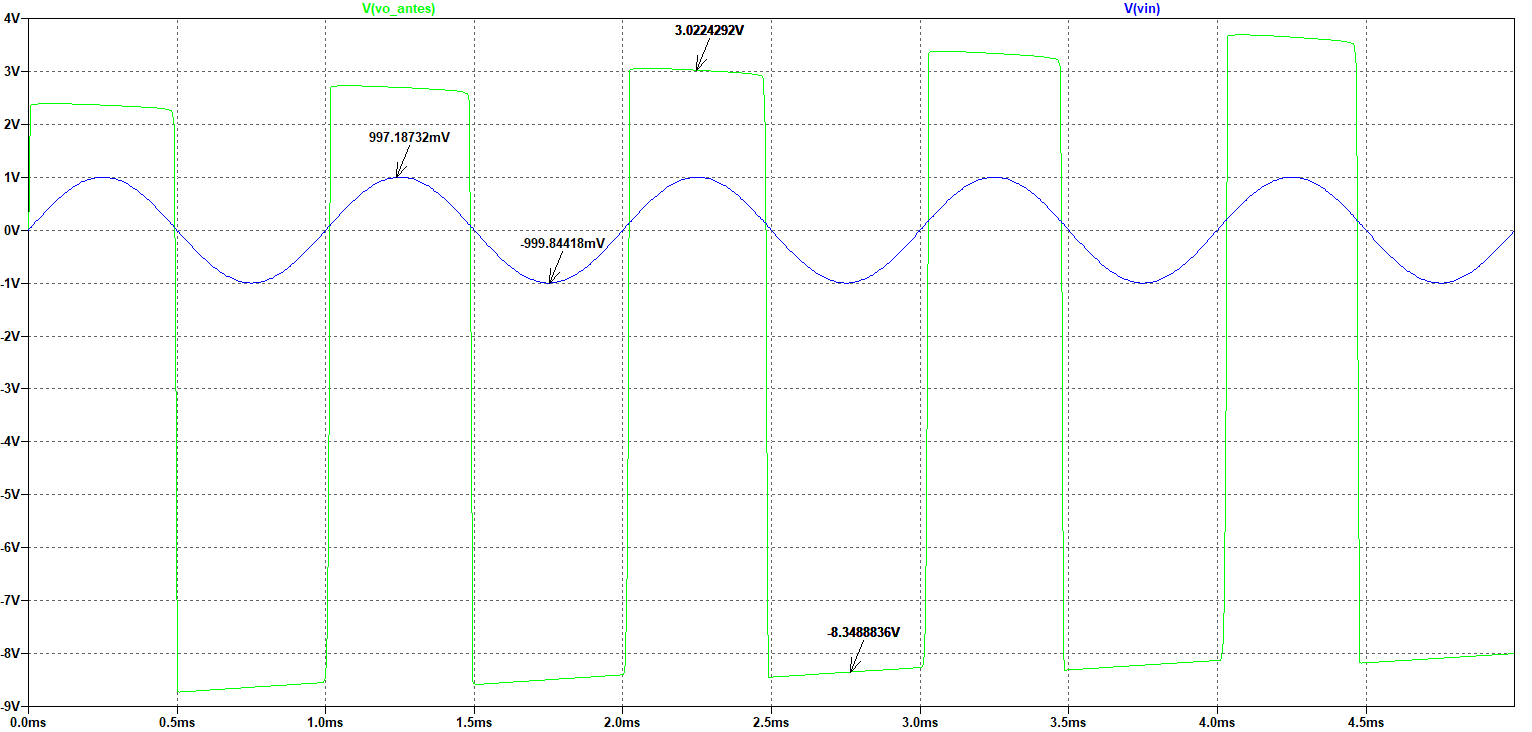
\includegraphics[width=\textwidth]{Imagenes/sim_base_1.png}
                  \caption{Simulación del voltaje de salida y entrada del amplificador base en tiempo con un $V_{in}=1V_p$ en modo diferencial.}
                  \label{fig:sim_base_1}
                \end{figure}

                Se puede observar en la figura \ref{fig:sim_base_1}, que si hallamos la ganancia daría lo siguiente:

                \begin{align*}
                  A_v & =\dfrac{3.022429-(-8.348883)}{997.18732m-(-999.84418m)} \\[0.2cm]
                  A_v & =5.7                                                    \\[0.2cm]
                \end{align*}

                Sin embargo como tiene una ganancia de 378.84, tenemos la salida saturada, como se puede observar, en ese caso usamos un voltaje de entrada de $1m\volt$, como se observa en la figura \ref{fig:sim_base_1m}.

                \begin{figure}[H]
                  \centering
                  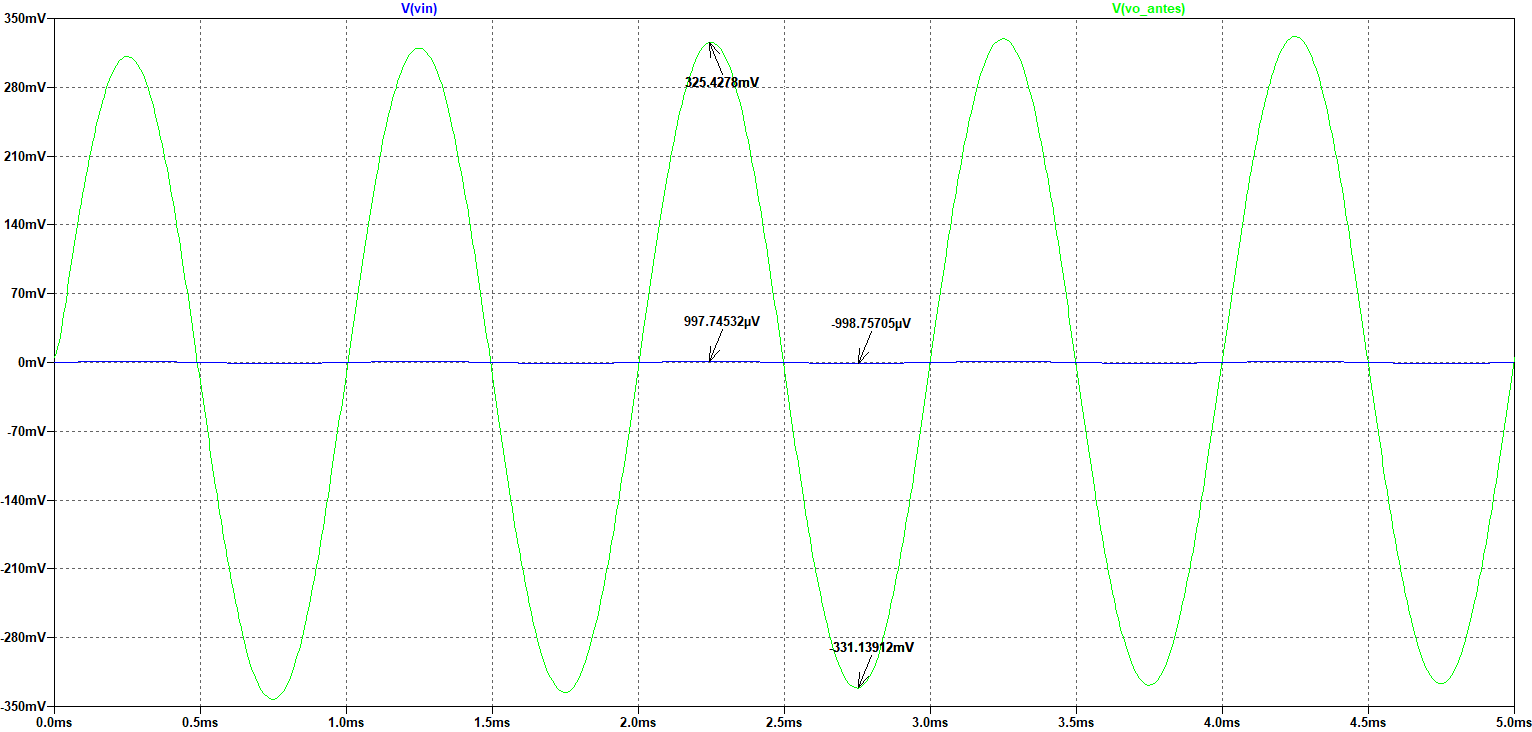
\includegraphics[width=\textwidth]{Imagenes/sim_base_1m.png}
                  \caption{Simulación del voltaje de salida y entrada del amplificador base en tiempo con un $V_{in}=1mV_p$ en modo diferencial.}
                  \label{fig:sim_base_1m}
                \end{figure}

                Acá si podemos ver que no existe una saturación y debido a esto si se ve su verdadera ganancia que seria la siguiente:

                \begin{align*}
                  A_v & =\dfrac{325.4278m-(-331.13912)}{997.74532\mu-(-998.75705\mu)} \\[0.2cm]
                  A_v & =328.86                                                       \\[0.2cm]
                \end{align*}

                Nos da una ganancia aproximada a la calculada, por hallarse en la zona activa, verificando de esa manera que hemos hecho unos cálculos teóricos adecuados.
                \newpage
          \item \textbf{Ganancia de tensión modo Común}

                \begin{figure}[H]
                  \centering
                  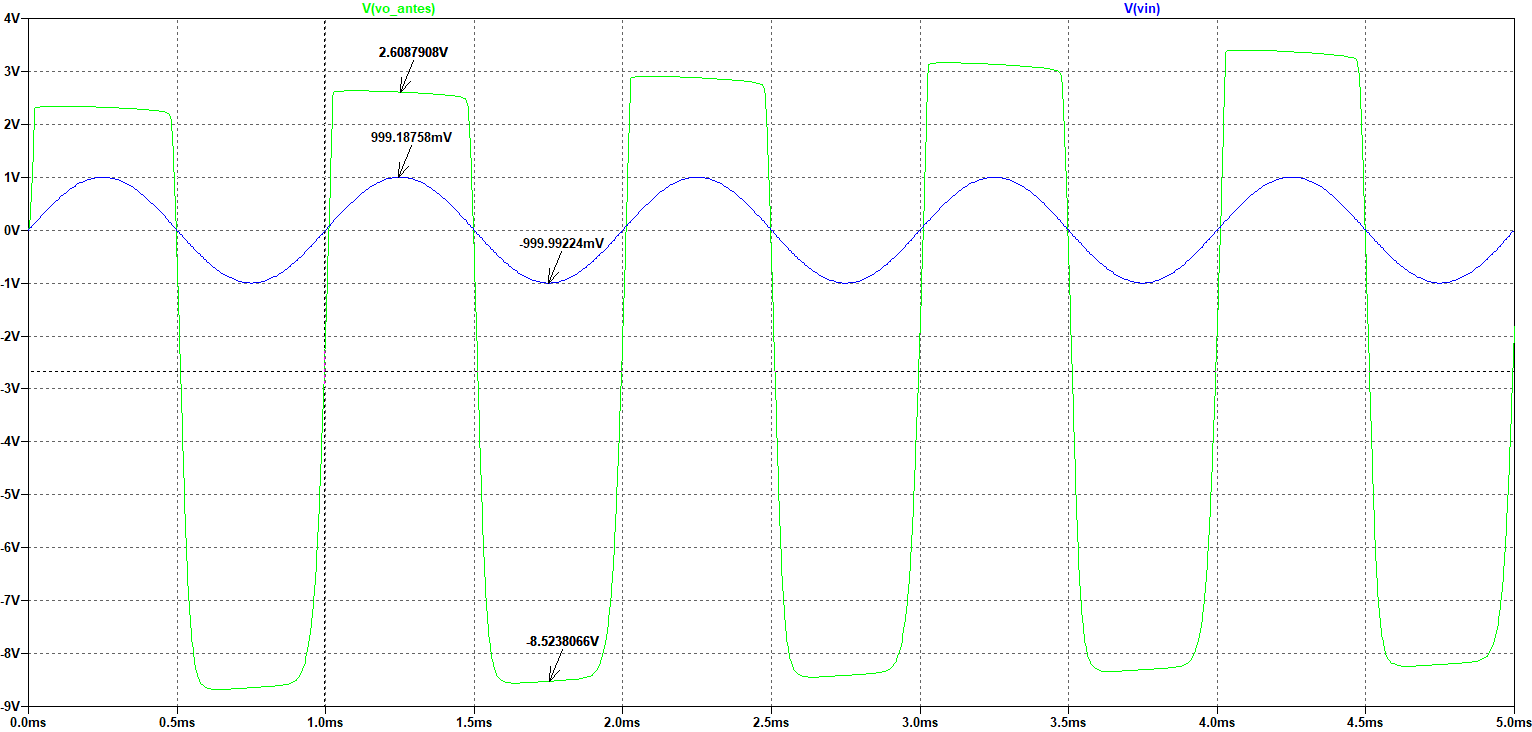
\includegraphics[width=\textwidth]{Imagenes/sim_basecomun_1.png}
                  \caption{Simulación del voltaje de salida y entrada del amplificador base en tiempo con un $V_{in}=1V_p$ en modo común.}
                  \label{fig:sim_basecomun_1}
                \end{figure}

                Se puede observar en la figura \ref{fig:sim_basecomun_1}, que si hallamos la ganancia daría lo siguiente:

                \begin{align*}
                  A_c & =\dfrac{2.6087908-(-8.5238066)}{999.18758m-(-999.99224m)} \\[0.2cm]
                  A_c & =5.6                                                      \\[0.2cm]
                \end{align*}

                Sin embargo como tiene una ganancia de 27.91, tenemos la salida saturada, como se puede observar, en ese caso usamos un voltaje de entrada de $1m\volt$, como se observa en la figura \ref{fig:sim_basecomun_1m}. Si nos fijamos da igual que la ganancia de tensión en modo diferencial, debido a su polarización que se mantienen iguales.

                \begin{figure}[H]
                  \centering
                  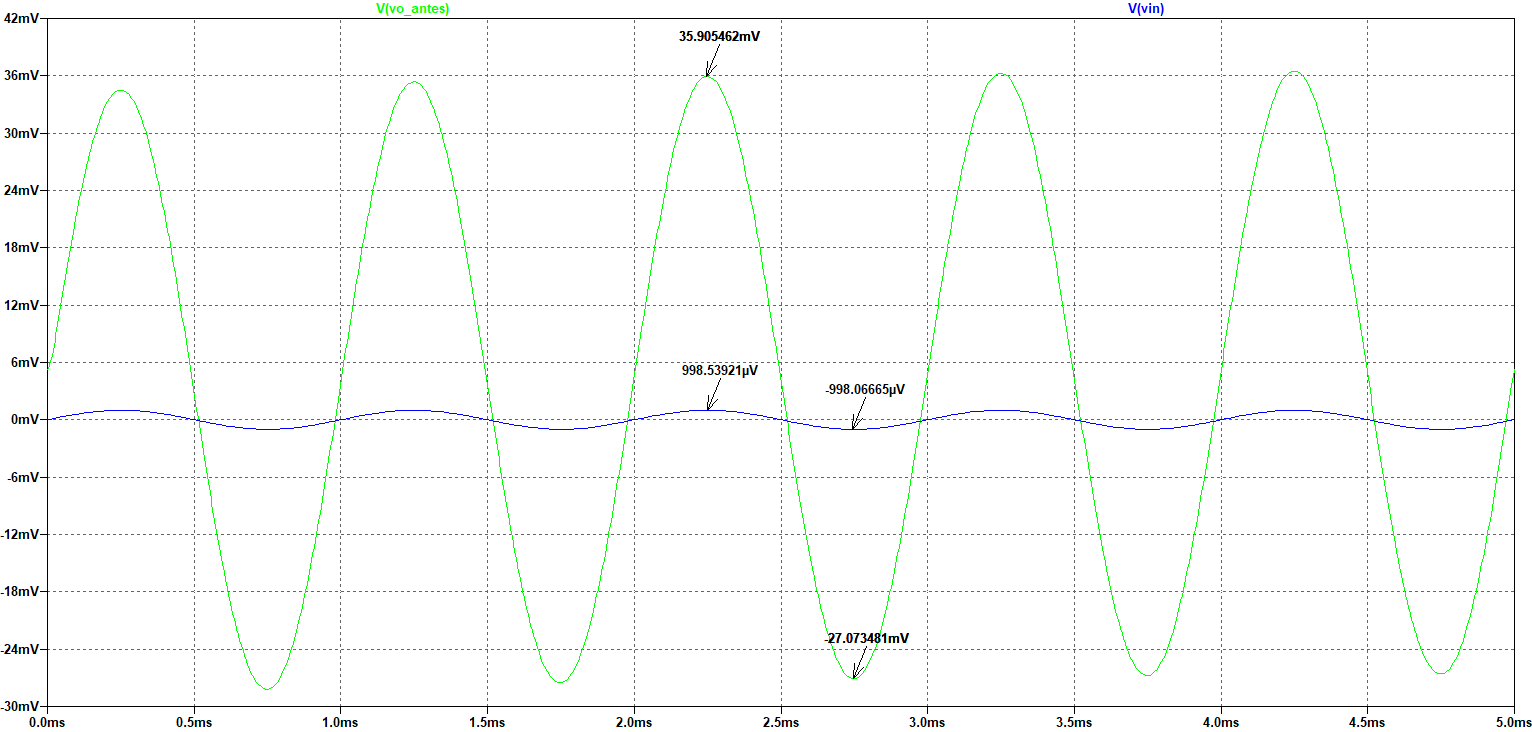
\includegraphics[width=\textwidth]{Imagenes/sim_basecomun_1m.png}
                  \caption{Simulación del voltaje de salida y entrada del amplificador base en tiempo con un $V_{in}=1mV_p$ en modo común.}
                  \label{fig:sim_basecomun_1m}
                \end{figure}

                \begin{align*}
                  A_c & =\dfrac{35.905462m-(-27.073481m)}{998.53921\mu-(-998.06665\mu)} \\[0.2cm]
                  A_c & =31.54                                                          \\[0.2cm]
                \end{align*}

                Nos da una ganancia aproximada a la calculada, por hallarse en la zona activa, verificando de esa manera que hemos hecho unos cálculos teóricos adecuados.

                Cada uno de los resultados pueden compararse con la tabla \ref{tab:dinamico_base}.

          \item  \textbf{Impedancia de entrada modo Diferencial}

                Haremos uso de la ecuación \ref{eqn:zd}, tras la simulación usar los valores dados por ello.

                \begin{figure}[H]
                  \centering
                  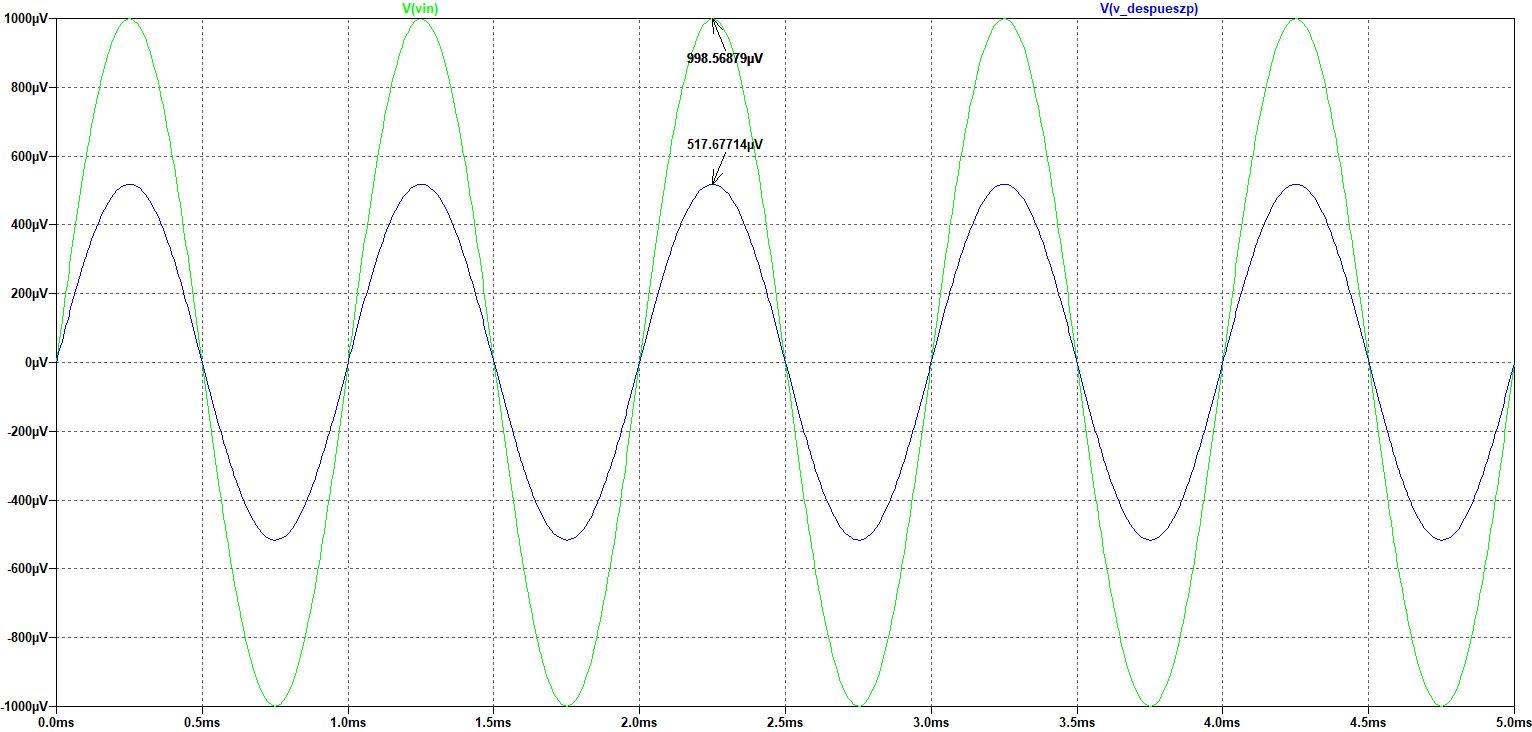
\includegraphics[width=\textwidth]{Imagenes/sim_base_zd.png}
                  \caption{Simulación del voltaje de entrada y después de $Z_p$ en modo común, para hallar $Z_d$.}
                  \label{fig:sim_base_zd}
                \end{figure}

                \begin{align*}
                  Z_{d} & =\dfrac{V_{despues\_de\_Z\_p}Z_p}{V_{in}-V_{despues\_de\_Z\_p}} \\[0.2cm]
                  Z_{d} & =\dfrac{517.67714\mu(42k)}{998.56879\mu-517.67714\mu}           \\[0.2cm]
                  Z_{d} & =45.212k\ohm                                                    \\[0.2cm]
                \end{align*}

          \item  \textbf{Impedancia de entrada modo Común}

                Haremos uso de la ecuación \ref{eqn:zc}, tras la simulación usar los valores dados por ello.


                \begin{figure}[H]
                  \centering
                  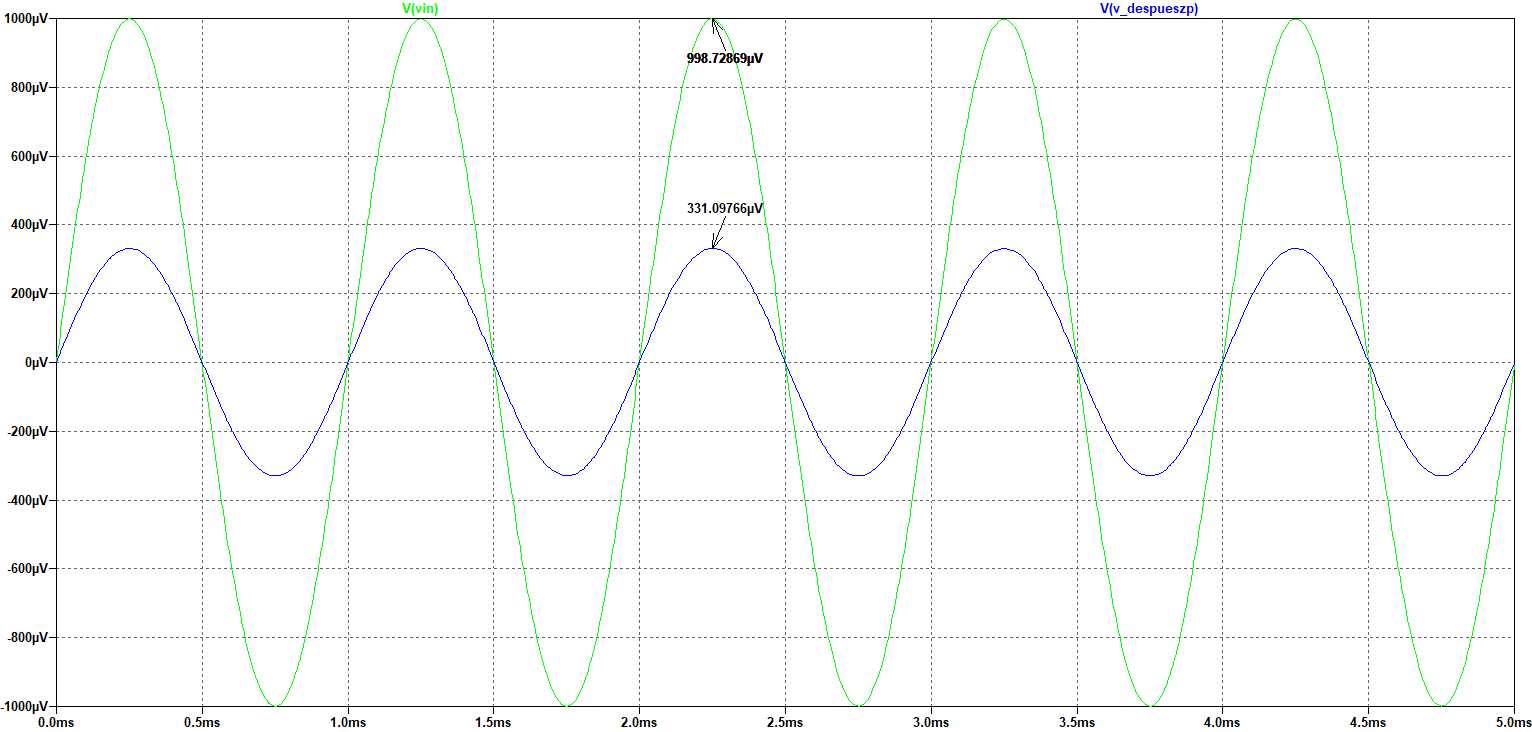
\includegraphics[width=\textwidth]{Imagenes/sim_base_zc.png}
                  \caption{Simulación del voltaje de entrada y después de $Z_p$ en modo común, para hallar $Z_c$.}
                  \label{fig:sim_base_zc}
                \end{figure}

                \begin{align*}
                  Z_{c} & =2\dfrac{V_{despues\_de\_Z\_p}Z_p}{V_{in}-V_{despues\_de\_Z\_p}} \\[0.2cm]
                  Z_{c} & =2\dfrac{517.67714\mu(50k)}{998.56879\mu-517.67714\mu}           \\[0.2cm]
                  Z_{c} & =49.6k\ohm                                                       \\[0.2cm]
                \end{align*}

          \item  \textbf{Impedancia de salida}

                En este apartado, se va a establecer la impedancia de salida con la ecuación \ref{eqn:zo}, pero bajo las simulaciones realizadas previamente para la metodología adecuada del laboratorio.

                \begin{figure}[H]
                  \centering
                  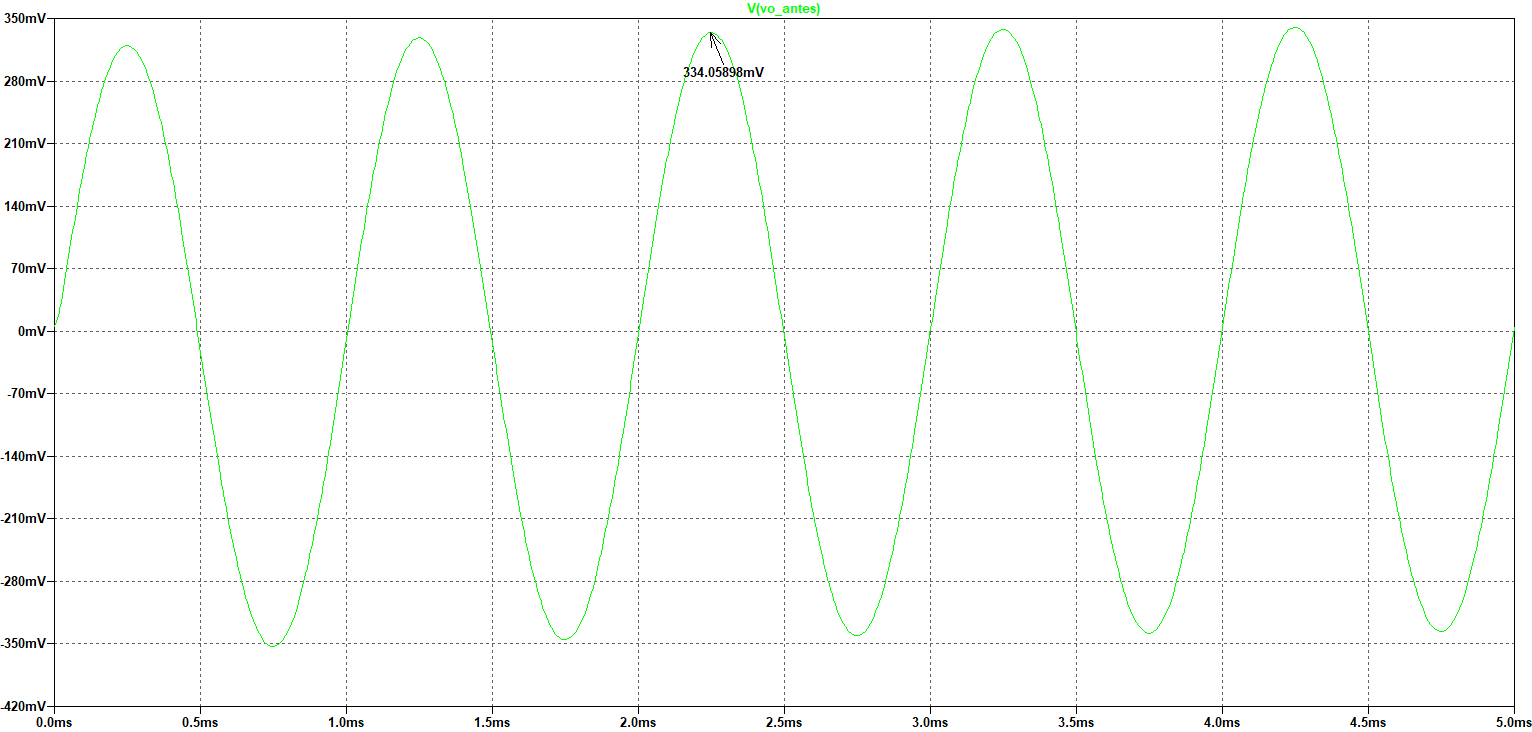
\includegraphics[width=\textwidth]{Imagenes/vosc_base.png}
                  \caption{Simulación del voltaje de salida sin carga del amplificador base en tiempo para hallar la impedancia de salida.}
                  \label{fig:vosc_base}
                \end{figure}

                En la figura \ref{fig:vosc_base}, se visualiza el voltaje de salida sin carga, ahora se usara el valor de la simulación de la figura \ref{fig:vocc_base}, y hallar la impedancia de salida.

                \begin{figure}[H]
                  \centering
                  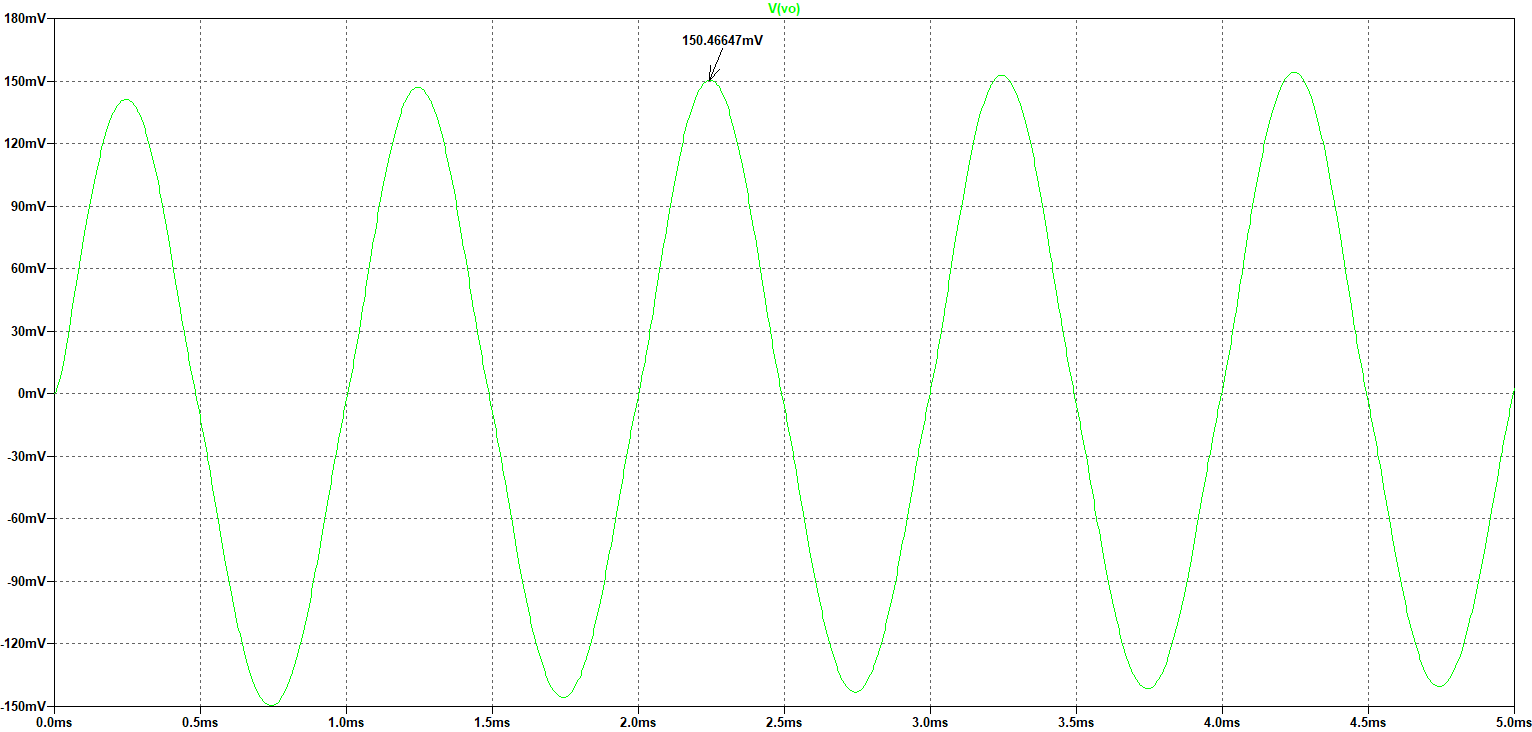
\includegraphics[width=\textwidth]{Imagenes/vocc_base.png}
                  \caption{Simulación del voltaje de salida con carga del amplificador base en tiempo para hallar la impedancia de salida.}
                  \label{fig:vocc_base}
                \end{figure}

                \begin{align*}
                  Z_{out} & =\dfrac{(V_{sin\_carga}-V_{con\_carga})Z_p}{V_{con\_carga}} \\[0.2cm]
                  Z_{out} & =\dfrac{(334.05898m-150.46647m)30}{150.46647m}              \\[0.2cm]
                  Z_{out} & =36.6\ohm                                                   \\[0.2cm]
                \end{align*}

        \end{itemize}

        \begin{table}[H]
          \centering
          \begin{tabular}{|c|c|c|c|c|}
            \hline
            $\mathbf{A_d}$ & $\mathbf{A_c}$ & $\mathbf{Z_{d}[\ohm]}$ & $\mathbf{Z_{c}[\ohm]}$ & $\mathbf{Z_{out} [\ohm]}$ \\ \hline
            5.7            & 5.6            & 45.212k                & 49.593k                & 36.6                      \\ \hline
          \end{tabular}
          \captionsetup{labelfont={bf}}
          \caption{Ganancia e impedancias simuladas del amplificador base con un $V_{in}=1V_p$}
          \label{tab:dinamico_base_sim1}
        \end{table}

        \begin{table}[H]
          \centering
          \begin{tabular}{|c|c|c|c|c|}
            \hline
            $\mathbf{A_d}$ & $\mathbf{A_c}$ & $\mathbf{Z_{d}[\ohm]}$ & $\mathbf{Z_{c}[\ohm]}$ & $\mathbf{Z_{out} [\ohm]}$ \\ \hline
            328.86         & 34.54          & 45.212k                & 49.593k                & 36.6                      \\ \hline
          \end{tabular}
          \captionsetup{labelfont={bf}}
          \caption{Ganancia e impedancias simuladas del amplificador base con un $V_{in}=1mV_p$}
          \label{tab:dinamico_base_sim1m}
        \end{table}

\end{enumerate}


\subsection{Parte 4. Respuesta en frecuencia}

\begin{enumerate}
  \item \textbf{Para el amplificador base (figura \ref{fig:amplificador_base}), determine: Punto
          de operación de los elementos activos y modelo dinámico del amplificador, incluyendo su respuesta en frecuencia.}

        Los datos de los puntos de operación y modelo dinámico se encuentran en las tablas \ref{tab:ptos_ed}, \ref{tab:ptos_ei}, \ref{tab:ptos_ep} y \ref{tab:dinamico_base}.

        Se hará énfasis en su respuesta en frecuencia

        \subsubsection{Frecuencia de corte inferior}

        \begin{itemize}
          \item $\mathbf{C_1}$ y $\mathbf{C_3}$

                Se toman $C_1$ y $C_3$ como iguales, debido a que es el mismo recorrido de corriente en la etapa diferencial, uno es de acople y el otro de desacople.

                Se aplica el método de respuesta en frecuencia para corte inferior, se obtiene el siguiente circuito de la figura \ref{fig:c1}
                \begin{figure}[H]
                  \centering
                  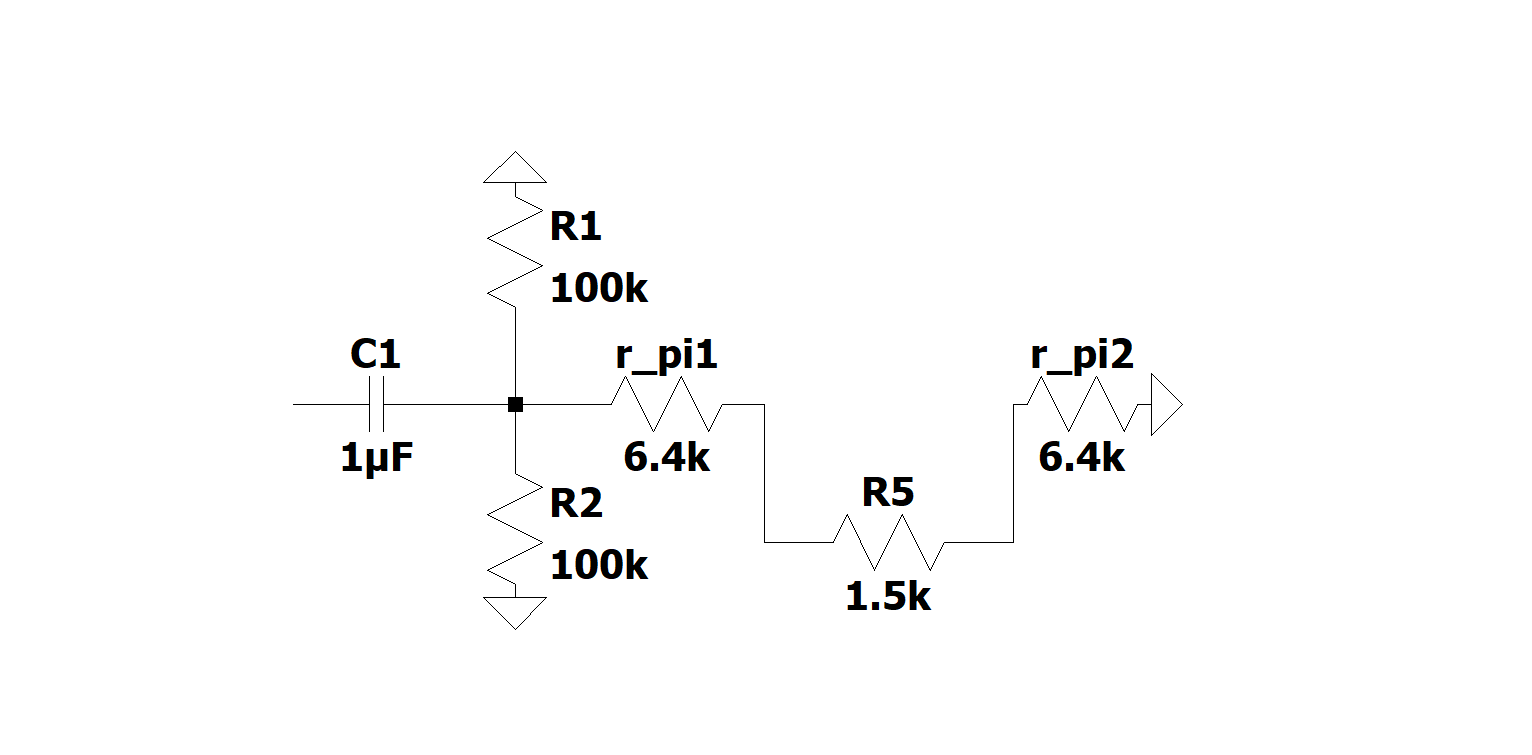
\includegraphics[width=12cm]{Imagenes/c1.png}
                  \caption{Diagrama esquemático al aplicar el análisis de frecuencia de corte inferior a $C_1$.}
                  \label{fig:c1}
                \end{figure}

                Se halla la $Z_{eq}$ del circuito de la figura \ref{fig:c1}, dando como resultado lo siguiente,

                Aplicando la ecuación \ref{eqn:wl}.

                \begin{align*}
                  w_{p_1} & =w_{p_3}=\dfrac{1}{C_1Z_{eq}}                                                                                    \\[0.2cm]
                  w_{p_1} & =\dfrac{1}{C_1[R_1||R_2||(r_{\pi_1}+(g_{m_1}r_{\pi_1}+1)\left(R_5+\dfrac{r_{\pi_2}}{g_{m_2}r_{\pi_2}+1}\right)]} \\[0.2cm]
                  w_{p_1} & =\dfrac{1}{C_1[R_1||R_2||(2r_{\pi_1}+(g_{m_1}r_{\pi_1}+1)\left(R_5\right)]}                                      \\[0.2cm]
                  w_{p_1} & =w_{p_3}= \SI{24.18}{\radian\per\second}                                                                         \\[0.2cm]
                  f_{L_1} & =f_{L_3}= \SI{3.85}{\hertz}                                                                                      \\[0.2cm]
                \end{align*}

          \item $\mathbf{C_2}$

                \begin{figure}[H]
                  \centering
                  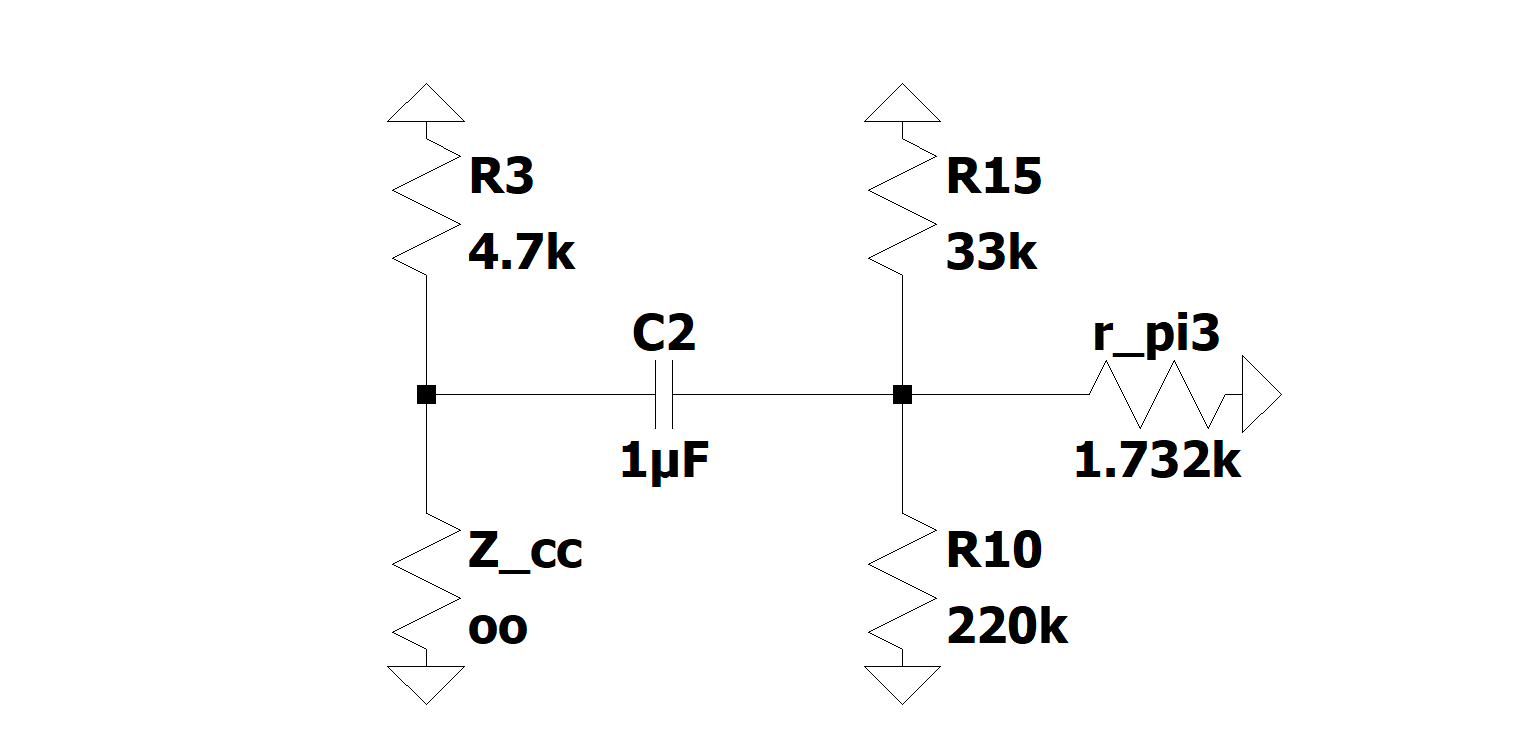
\includegraphics[width=12cm]{Imagenes/c2.png}
                  \captionsetup{labelfont={bf}}
                  \caption{Diagrama esquemático al aplicar el análisis de frecuencia de corte inferior a $C_2$.}
                  \label{fig:c2}
                \end{figure}

                Se halla la $Z_{eq}$ del circuito de la figura \ref{fig:c2}, dando como resultado lo siguiente,

                \begin{align*}
                  w_{p_2} & =\dfrac{1}{C_2Z_{eq}}                            \\[0.2cm]
                  w_{p_2} & =\dfrac{1}{C_2[R_3+(R_{15}||R_{10}||r_{\pi_3})]} \\[0.2cm]
                  w_{p_2} & = \SI{157.9}{\radian\per\second}                 \\[0.2cm]
                  f_{L_2} & = \SI{25.13}{\hertz}                             \\[0.2cm]
                \end{align*}

          \item $\mathbf{C_5}$

                \begin{figure}[H]
                  \centering
                  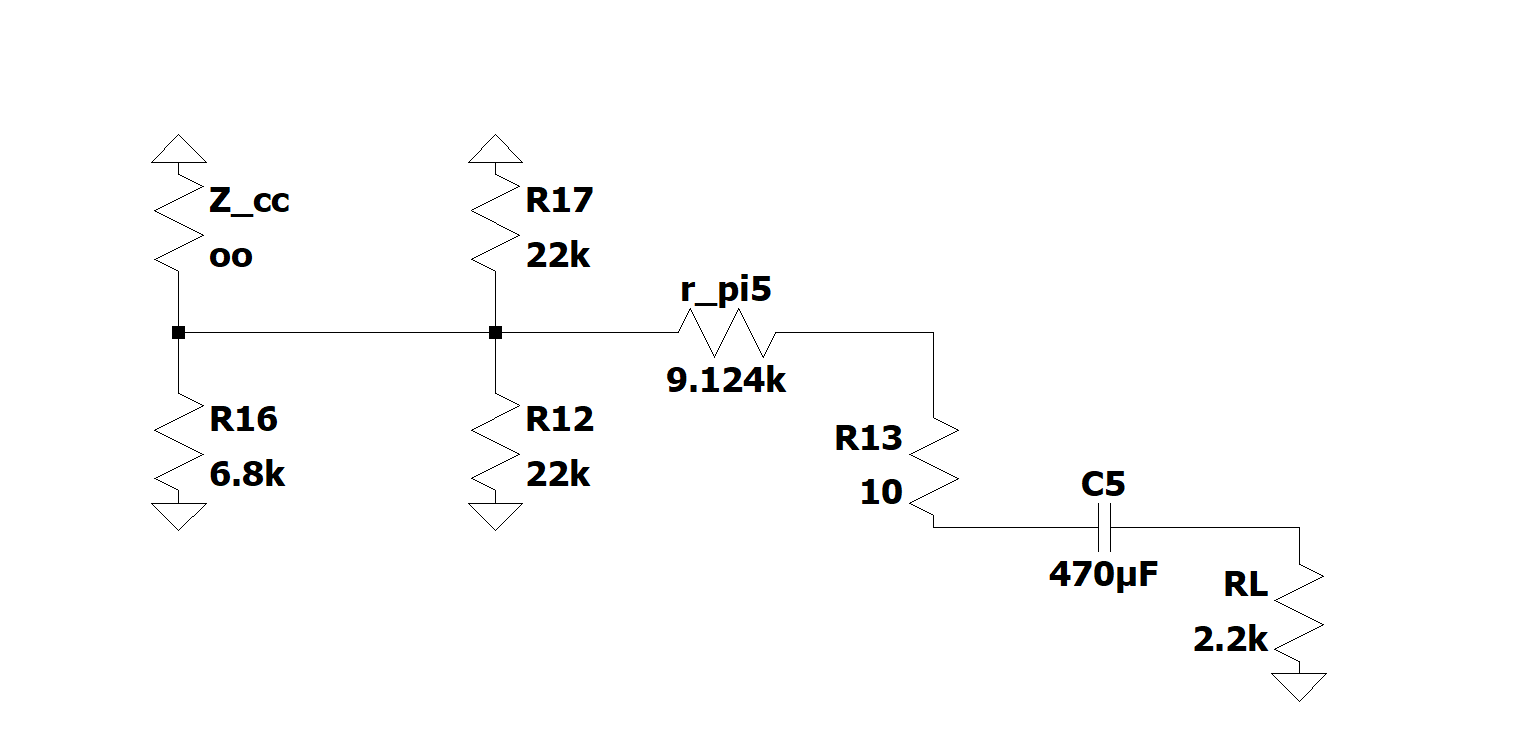
\includegraphics[width=12cm]{Imagenes/c5.png}
                  \captionsetup{labelfont={bf}}
                  \caption{Diagrama esquemático al aplicar el análisis de frecuencia de corte inferior a $C_5$.}
                  \label{fig:c5}
                \end{figure}

                Se halla la $Z_{eq}$ del circuito de la figura \ref{fig:c5}, dando como resultado lo siguiente,

                \begin{align*}
                  w_{p_5} & =\dfrac{1}{C_5Z_{eq}}                                                                               \\[0.2cm]
                  w_{p_5} & =\dfrac{1}{C_5[R_L+R_{13}+\dfrac{r_{\pi_5}+R_{17}||R_{12}||R_{16}||Z_{CCQ_3}}{g_{m_5}r_{\pi_5}+1}]}
                \end{align*}


                En este caso, para $Z_{CCQ_3}$ que es la impedancia vista desde el colector hacia el transistor, se facilita la obtención del valor, a través del transistor completamente cargado, donde se obtiene la siguiente ecuación:

                \begin{gather*}
                  Z_{CCQ_3}=r_o \left[\dfrac{r_{\pi}+Z_B+\left(g_mr_{\pi}+1+\dfrac{r_{\pi}+Z_B}{r_o}\right)Z_E}{Z_E+Z_B+r_{\pi}}\right]
                \end{gather*}

                Donde, $Z_B$, es la impedancia vista desde la base y $Z_E$, es la impedancia vista desde el emisor.

                Como se puede observar, $Z_E=0$ por el condensador, por ende, la ecuación generada por el transistor completamente cargado solo nos quedaría $Z_{CCQ_3}=r_o$, de esa manera se obtiene la siguiente frecuencia de $C_5$
                \begin{align*}
                  w_{p_5} & =\dfrac{1}{C_5[R_L+R_{13}+\dfrac{r_{\pi_5}+R_{17}||R_{12}||R_{16}||r_{o_3}}{g_{m_5}r_{\pi_5}+1}]}
                  w_{p_5} & = \SI{0.096}{\radian\per\second}                                                                  \\[0.2cm]
                  f_{L_5} & = \SI{15.31}{\milli\hertz}                                                                        \\[0.2cm]
                \end{align*}
                \newpage
          \item $\mathbf{C_6}$

                \begin{figure}[H]
                  \centering
                  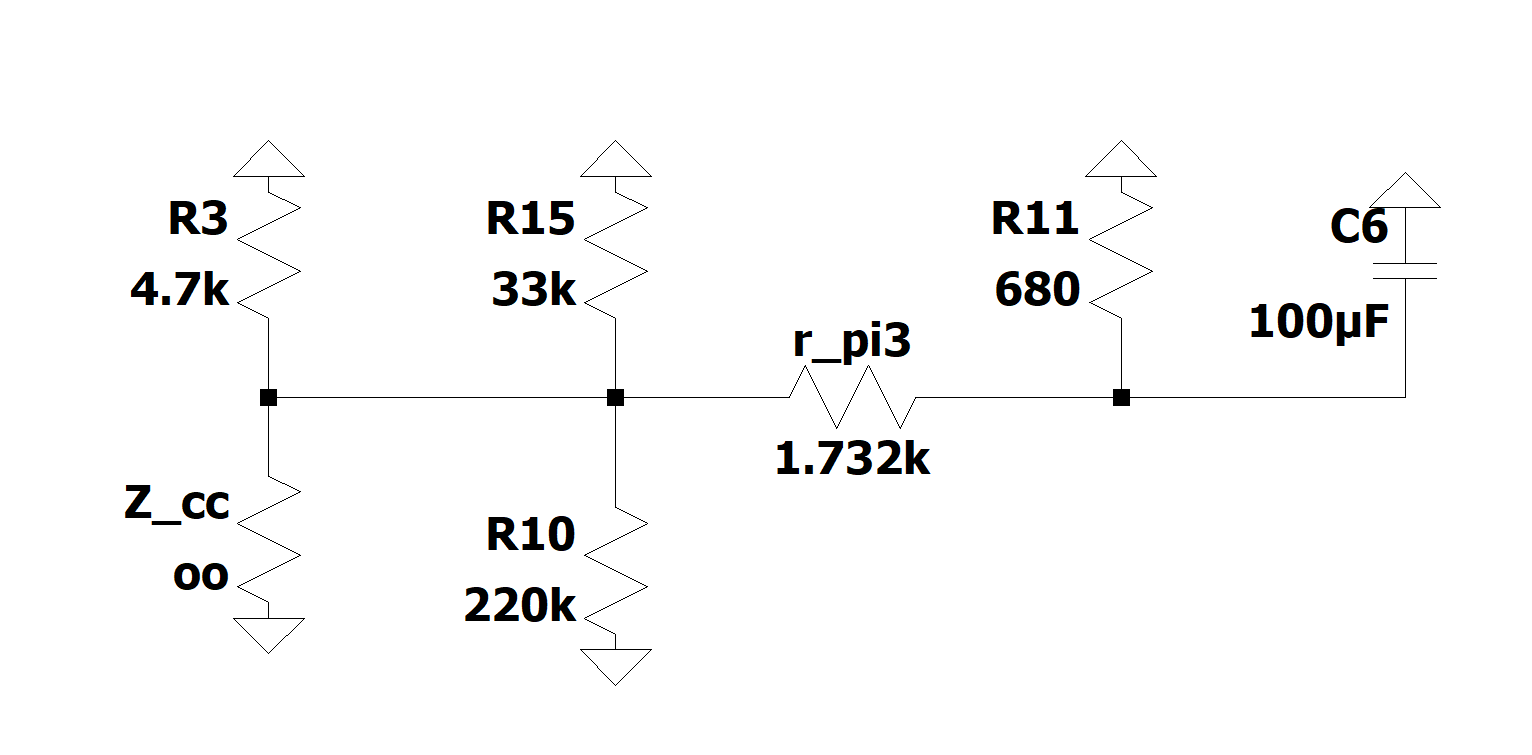
\includegraphics[width=12cm]{Imagenes/c6.png}
                  \captionsetup{labelfont={bf}}
                  \caption{Diagrama esquemático al aplicar el análisis de frecuencia de corte inferior a $C_6$.}
                  \label{fig:c6}
                \end{figure}

                Se halla la $Z_{eq}$ del circuito de la figura \ref{fig:c6}, dando como resultado lo siguiente,

                \begin{align*}
                  w_{p_6} & =\dfrac{1}{C_6Z_{eq}}                                                                             \\[0.2cm]
                  w_{p_6} & =\dfrac{1}{C_6[R_{11}||\left(\dfrac{r_{\pi_3}+R_{15}||R_{10}||R_{3}}{g_{m_3}r_{\pi_3}+1}\right)]} \\[0.2cm]
                  w_{p_6} & = \SI{277.22}{\radian\per\second}                                                                 \\[0.2cm]
                  f_{L_6} & = \SI{44.121}{\hertz}                                                                             \\[0.2cm]
                \end{align*}

          \item $\mathbf{C_7}$

                \begin{figure}[H]
                  \centering
                  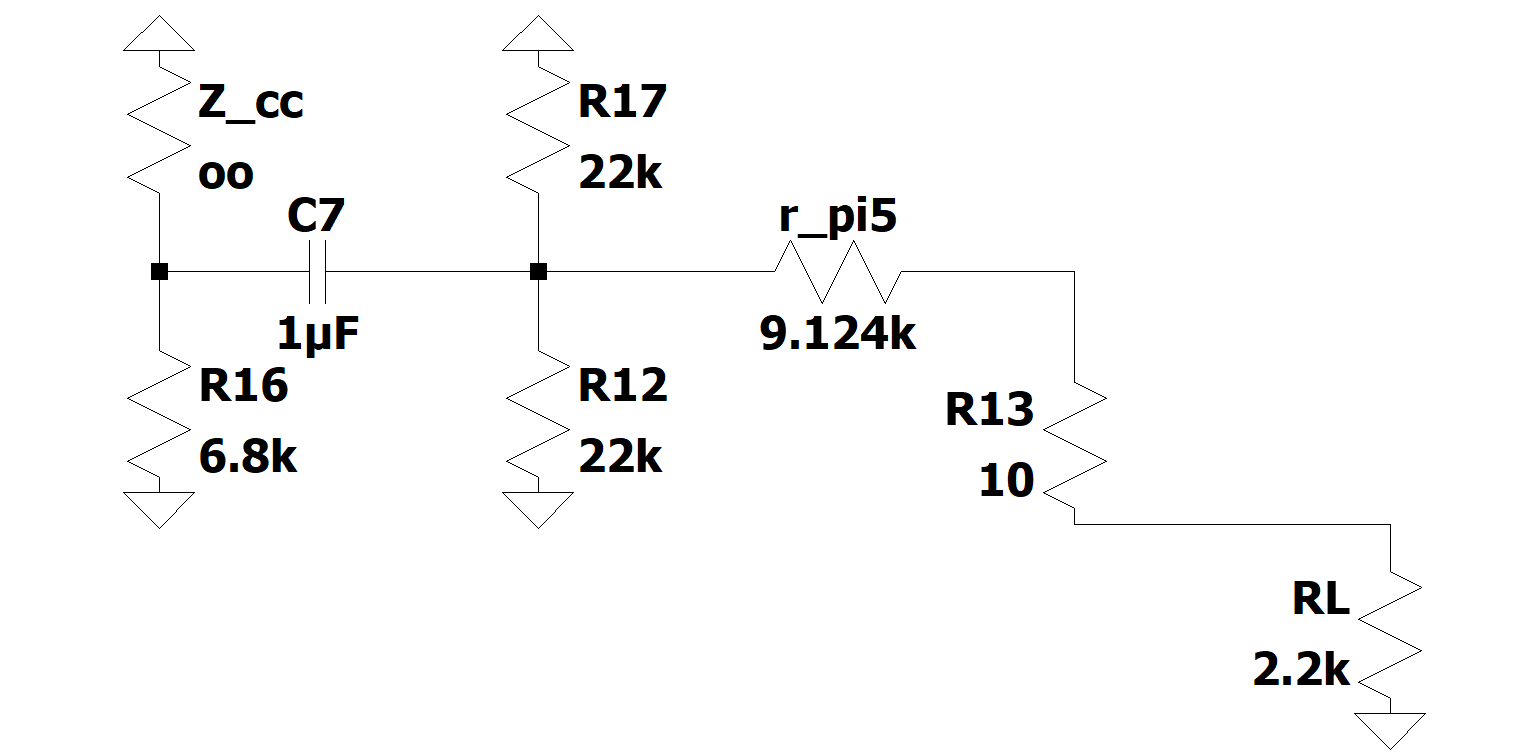
\includegraphics[width=12cm]{Imagenes/c7.png}
                  \captionsetup{labelfont={bf}}
                  \caption{Diagrama esquemático al aplicar el análisis de frecuencia de corte inferior a $C_7$.}
                  \label{fig:c7}
                \end{figure}

                Se halla la $Z_{eq}$ del circuito de la figura \ref{fig:c7}, dando como resultado lo siguiente,

                \begin{align*}
                  w_{p_7} & =\dfrac{1}{C_7Z_{eq}}                                                                \\[0.2cm]
                  w_{p_7} & =\dfrac{1}{C_7[R_{16}+R_{17}||R_{12}||(r_{\pi_5}+(g_{m_5}r_{\pi_5}+1)(R_{13}+R_L))]} \\[0.2cm]
                  w_{p_7} & = \SI{57.28}{\radian\per\second}                                                     \\[0.2cm]
                  f_{L_7} & = \SI{9.12}{\hertz}                                                                  \\[0.2cm]
                \end{align*}

                Como se pueden observar en los resultados, el capacitor mas dominante es el $\mathbf{C_6}$ siendo este el de bypass quien nos permite una mayor ganancia, teniendo sentido en los cálculos teóricos
        \end{itemize}

        \subsubsection{Frecuencia de corte superior}
        \begin{itemize}
          \item $\mathbf{C_4}$

                En este apartado tomaremos en cuenta el teorema de Miller y el análisis de frecuencia de corte superior, las ecuaciones que se usaran son \ref{eqn:C_eq} y \ref{eqn:wh}, bajo el modelo pi de altas frecuencias, como se muestra en la figura \ref{fig:c4}

                \begin{figure}[H]
                  \centering
                  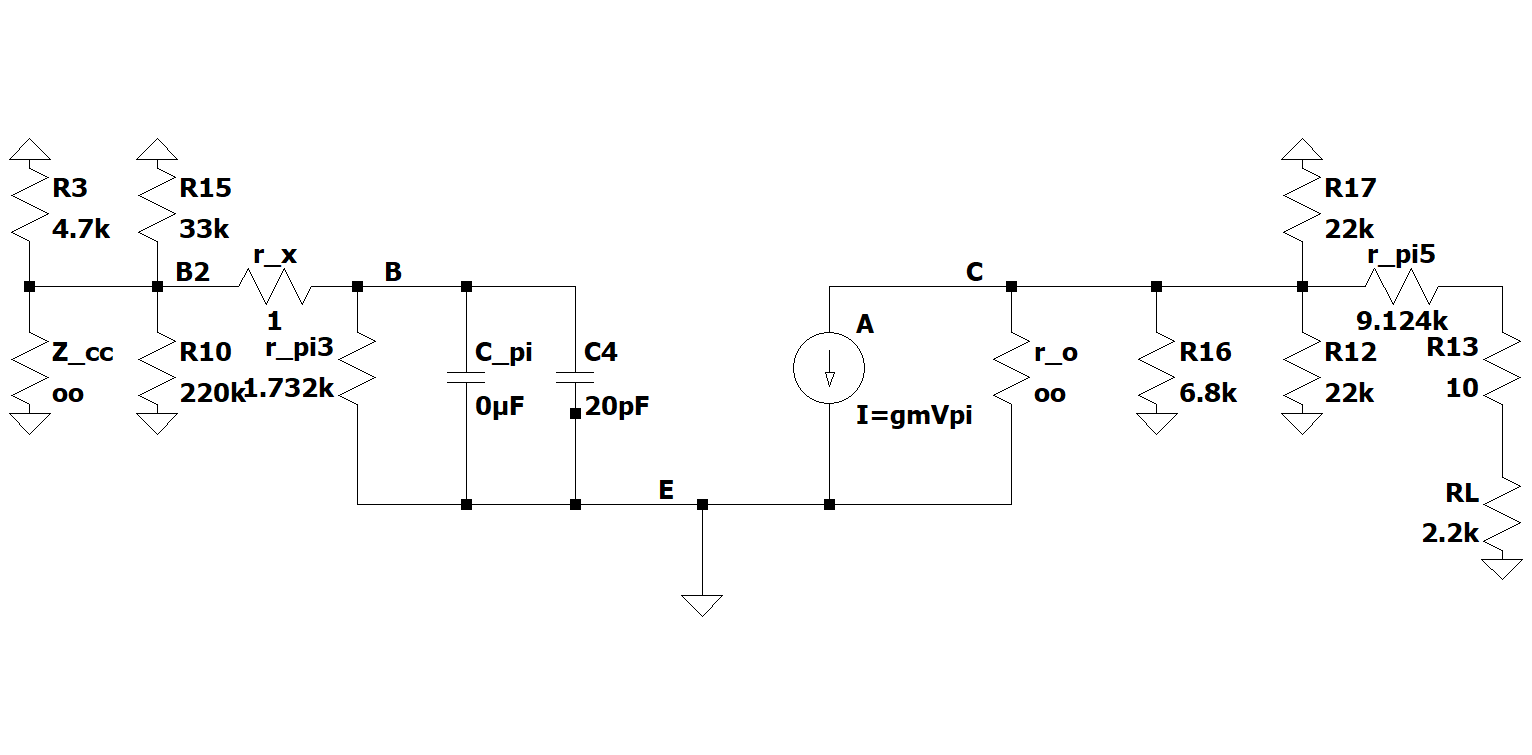
\includegraphics[width=\textwidth]{Imagenes/c4.png}
                  \captionsetup{labelfont={bf}}
                  \caption{Diagrama esquemático al aplicar el análisis de frecuencia de corte superior a $C_4$, aplicando Teorema de Miller.}
                  \label{fig:c4}
                \end{figure}

                \begin{align*}
                  \mathbf{C_{eq}} = C_{\pi} + C_{\mu}(1+g_mZ_{out})
                \end{align*}

                En este caso, se toma en cuenta el apartado de Anexos \ref{sec:anexos} donde se verifica que el transistor 2n3906 (PNP), el datasheet indica que $C_{\pi}=10 \, pF$ y $C_{\mu}=4.5 \, pF$, por lo tanto, se tiene que $C_{eq}$ es,

                \begin{align*}
                  \mathbf{C_{eq}} =C_{\pi}+ (C_{\mu}+C_4)(1+g_mZ_{out})
                \end{align*}

                Ahora, se halla $Z_{out}$ y sustituimos en \ref{eqn:C_eq},

                \begin{align*}
                  Z_{out} & =Z_{CCQ_3}||R_{16}||R_{17}||R_{12}||(r_{\pi_5}+(g_{m_5}r_{\pi_5}+1)(R_{13}+R_L))                                  \\[1cm]
                  C_{eq}  & =C_{\pi}+ (C_{\mu} + C_{4})(1+g_m[r_{o_3}||R_{16}||R_{17}||R_{12}||(r_{\pi_5}+(g_{m_5}r_{\pi_5}+1)(R_{13}+R_L))])
                \end{align*}

                Se toma en este caso, la ecuación \ref{eqn:rx}, donde se obtiene el valor de la resistencia de difusión;

                \begin{gather}
                  r_x=\dfrac{25.581 m}{2.253m}=11.35 \approx 11 \ohm
                \end{gather}


                luego se halla $Z_{in}$ y sustituimos en la ecuación \ref{eqn:wh}

                \begin{align*}
                  Z_{in} & =r_{\pi_3}||(r_{x}+(R_{15}||R_{10}||R_3))                                                                                                                                     \\[1cm]
                  w_{H}  & =\dfrac{1}{C_{eq}Z_{in}}                                                                                                                                                      \\[0.2cm]
                  w_{H}  & = \dfrac{1}{C_{\pi} + (C_{\mu} + C_{4})(1+g_{m_3}[r_{o_3}||R_{16}||R_{17}||R_{12}||(r_{\pi_5}+(g_{m_5}r_{\pi_5}+1)(R_{13}+R_L))]) [r_{\pi_3}||(r_{x}+(R_{15}||R_{10}||R_3))]} \\[0.2cm]
                  w_{H}  & =\SI{98.615}{\kilo\radian\per\second}                                                                                                                                         \\[0.2cm]
                  f_{H}  & =\SI{15.695}{\kilo\hertz}                                                                                                                                                     \\[0.2cm]
                \end{align*}

        \end{itemize}


        \begin{table}[H]
          \centering
          \begin{tabular}{|c|c|c|c|c|}
            \hline
            \textbf{Capacitores} & \boldmath{$\mathbf{w_L}$ (\si{\radian\per\second})} & \boldmath{$\mathbf{f_L}$ (\si{\hertz})} & \boldmath{$\mathbf{w_H}$ (\si{\radian\per\second})} & \boldmath{$\mathbf{f_H}$ (\si{\hertz})} \\\hline
            1                    & 24.18                                               & 3.85                                    & -                                                   & -                                       \\\hline
            2                    & 157.9                                               & 25.13                                   & -                                                   & -                                       \\\hline
            3                    & 24.18                                               & 3.85                                    & -                                                   & -                                       \\\hline
            4                    & -                                                   & -                                       & 98.615k                                             & 15.695k                                 \\\hline
            5                    & 0.096                                               & 15.31m                                  & -                                                   & -                                       \\\hline
            6                    & 277.22                                              & 44.121                                  & -                                                   & -                                       \\\hline
            7                    & 57.28                                               & 9.12                                    & -                                                   & -                                       \\\hline
          \end{tabular}
          \captionsetup{labelfont={bf}}
          \caption{Calculo teórico en el análisis de frecuencia de corte inferior y superior}
          \label{tab:frecuencias}
        \end{table}

        Como se puede observar en la frecuencia de corte inferior, el más dominante es la del capacitor $C_6$, siendo este el de bypass, debido a que permite una mayor ganancia, siendo el mas dominante en la frecuencia de baja, de esta manera sabemos que esa es la frecuencia de corte inferior.

        Por otro lado, tenemos el capacitor $C_4$ que es el que afecta en la frecuencia de corte superior, generando la frecuencia de corte superior como se observa en la tabla \ref{tab:frecuenciacorte}

        \begin{table}[H]
          \centering
          \begin{tabular}{|c|c|}
            \hline
            \boldmath{$\mathbf{f_L}$ (\si{\hertz})} & \boldmath{$\mathbf{f_H}$ (\si{\hertz})} \\\hline
            44.121                                  & 15.695k                                 \\\hline
          \end{tabular}
          \captionsetup{labelfont={bf}}
          \caption{Frecuencias de corte superior e inferior teórico}
          \label{tab:frecuenciacorte}
        \end{table}

  \item \textbf{Realice la simulación del circuito con el fin de verificar los cálculos previos.}

        \begin{figure}[H]
          \centering
          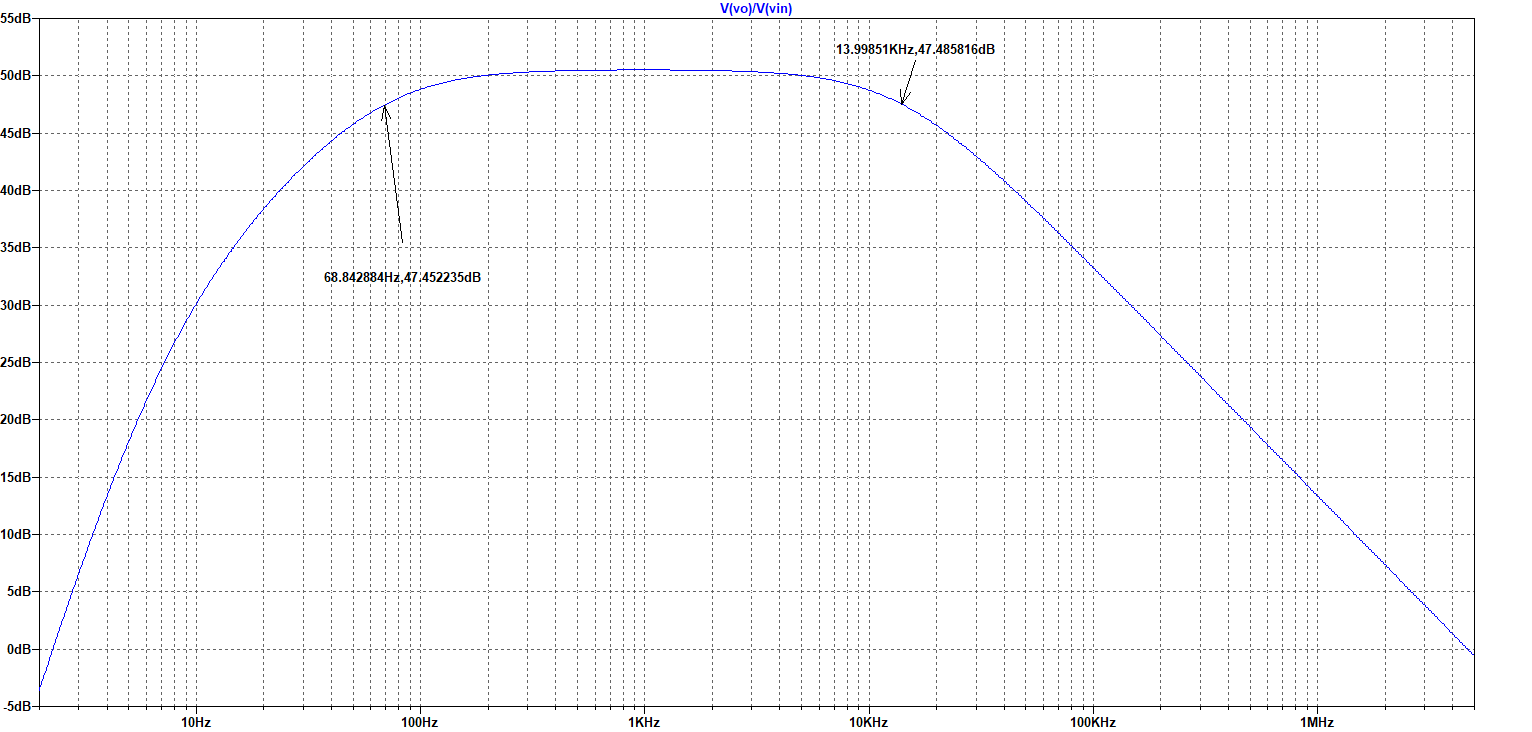
\includegraphics[width=\textwidth]{Imagenes/sim_resp_frecu.png}
          \captionsetup{labelfont={bf}}
          \caption{Simulación de la respuesta en frecuencia del amplificador base acoplando.}
          \label{fig:frecuenciacorte}
        \end{figure}

        \begin{figure}[H]
          \centering
          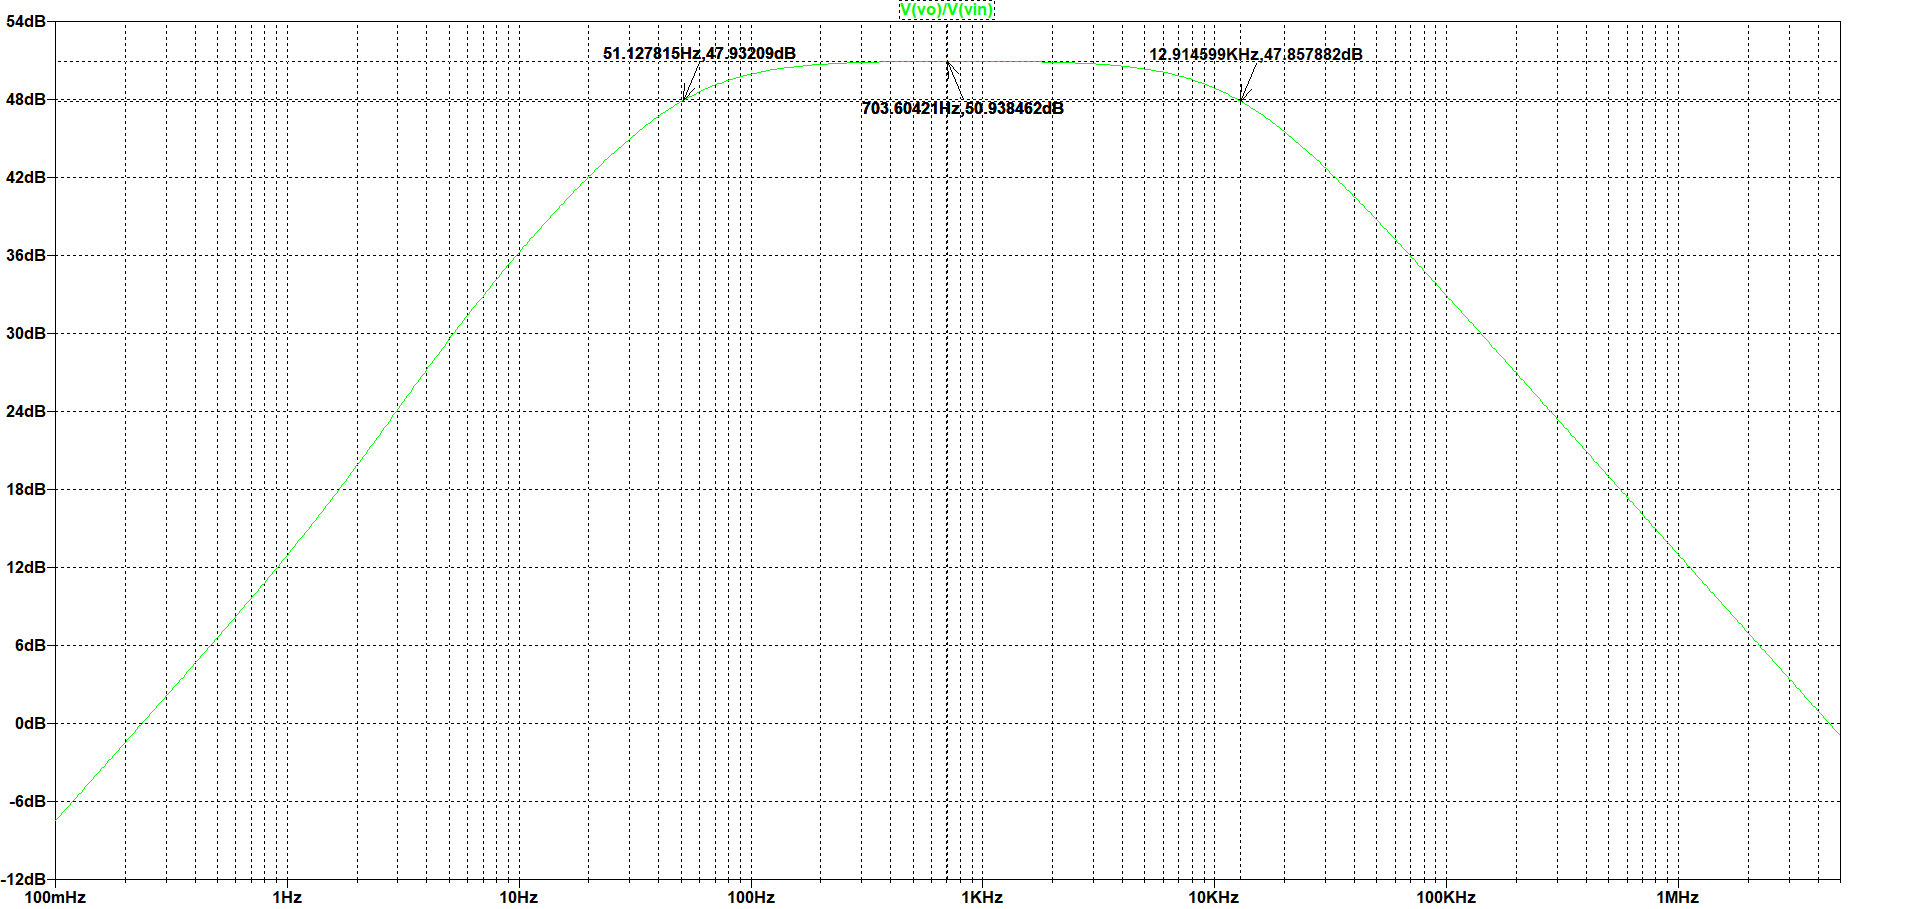
\includegraphics[width=\textwidth]{Imagenes/sim_resp_frecu_sin.png}
          \captionsetup{labelfont={bf}}
          \caption{Simulación de la respuesta en frecuencia del amplificador base sin acople de C2,C5,C7.}
          \label{fig:frecuenciacortesinacople}
        \end{figure}

        Como se puede observar los datos obtenidos de la simulación de la figura \ref{fig:frecuenciacorte} y \ref{fig:frecuenciacortesinacople}, en ambos casos se observa una ganancia aproximadamente cerca indicandonos que sea acoplado o desacoplado permitirá mantener su polarización
        obteniendo ganancias cercanas.

        Es importante recalcar que se puede hallar la frecuencia de corte total de la respuesta en frecuencia gracias a la ecuación \ref{eqn:wt}.

        \begin{align*}
          w_t & =\beta \cdot f_H         \\[0.2cm]
          w_t & =150 \cdot 15.695k       \\[0.2cm]
          w_t & =\SI{2.354}{\mega\hertz} \\[0.2cm]
        \end{align*}

        Nos da valores aproximados a los calculado, esto indica que los cálculos teóricos están bien realizados.

\end{enumerate}

\subsection{Parte 5. Realimentación}
\begin{enumerate}
  \item \textbf{Realimente negativamente el amplificador base a través de la entrada diferencial adecuada, mediante un divisor de tensión $R_f$ y $R_s$ , cuyos valores son los siguientes:}

        $$R_f=11k\ohm$$
        $$R_s=3.3k\ohm$$
        Para identificar de una manera más sencilla cual de las dos entradas de la etapa diferencial será la entrada positiva y negativa, podemos hacer el recorrido del amplificador base de la figura \ref{fig:amplificador_base}, primero desde una entrada y luego de la otra. El resultado final nos indicara si es positiva o negativa. Sin importar que este la fuente de voltaje en el nodo de la base del transistor 2. De esa manera, se tiene lo siguiente:

        Recorrido por $V_1$, que es donde tenemos la entrada de señal AC.

        Se recorre la base de $Q_1$ al colector de este mismo, que es donde se encuentra la salida de la etapa diferencial, cuando se va de base a colector la ganancia es negativa, debido a su modelo pi.

        $$A_1=-A_1$$

        Luego tenemos de base a colector de $Q_2$, que como se indico anteriormente que la ganancia sera negativa.

        $$A_2=-A_2$$

        Finalmente, tenemos $Q_3$ que va de base a emisor, que en este caso, dá una ganancia positiva.

        $$A_3=A_3$$

        Hallando la ganancia total del amplificador multietapas, dá el siguiente signo.
        $$A_V=-A_1(-A_2)A_3>0$$

        Por ende, donde se encuentra la señal de entrada es la entrada positiva del amplificador, por consiguiente, la entrada donde se encuentra la fuente negativa, es la entrada negativa. No por que posee una fuente negativa ocurre eso, sino por el estudio hecho anteriormente.

        En la figura \ref{fig:realimentadon} que se verá a continuación se tendrá el circuito realimentado por la entrada $V_2$, que seria la entrada inversora.

        \begin{figure}[H]
          \centering
          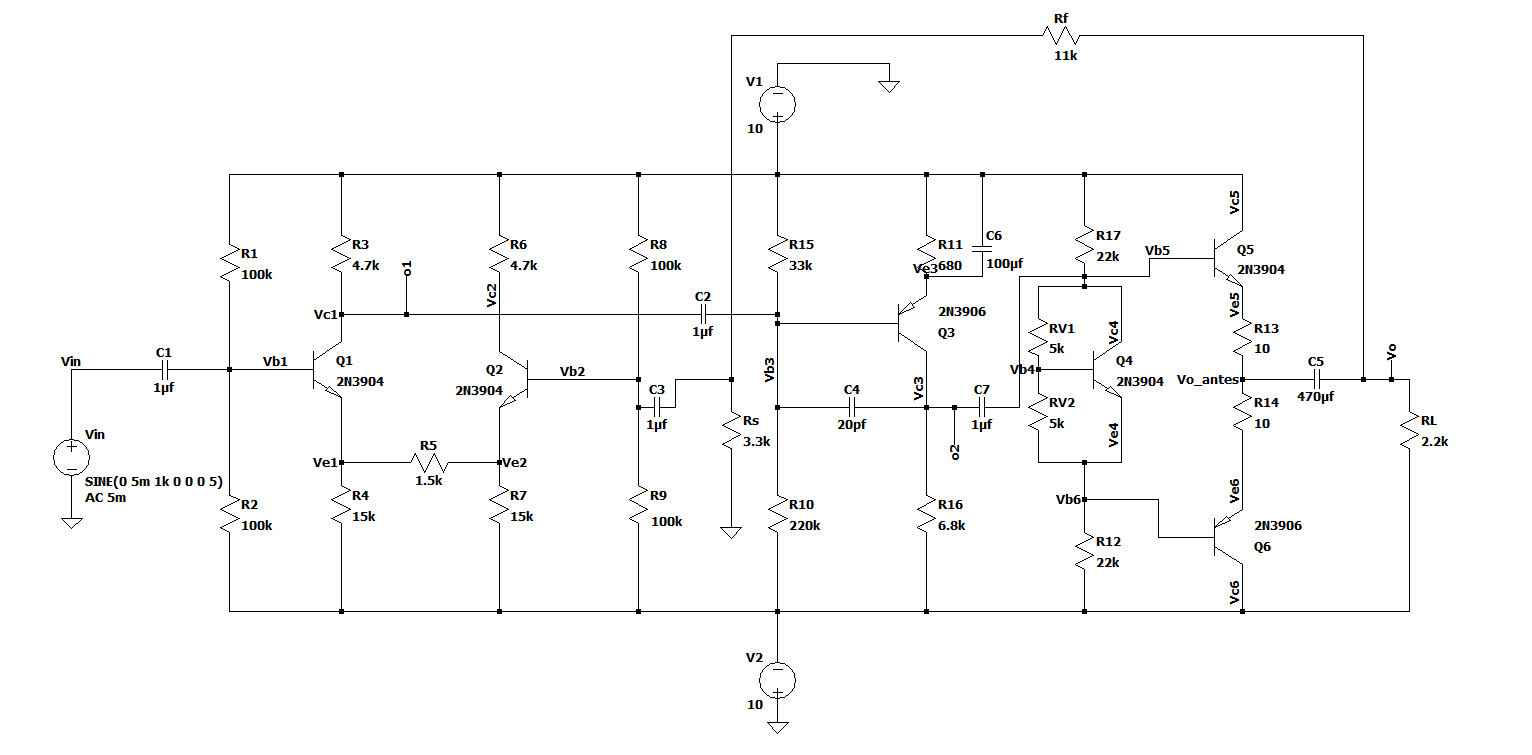
\includegraphics[width=\textwidth]{Imagenes/realimentado.png}
          \captionsetup{labelfont={bf}}
          \caption{Diagrama esquemático del amplificador base realimentado negativamente.}
          \label{fig:realimentadon}
        \end{figure}

  \item \textbf{Para el amplificador realimentado, determine: Puntos de operación de los elementos activos, el modelo dinámico del amplificador y su respuesta en frecuencia, utilizando la entrada libre del diferencial como entrada.}

        Los datos de los puntos de operación y modelo dinámico , no cambian, por ende, se encuentran en las tablas \ref{tab:ptos_ed}, \ref{tab:ptos_ei}, \ref{tab:ptos_ep} y \ref{tab:dinamico_base} .

        Sin embargo su respuesta en frecuencia si cambian, se realizará su estudio a continuación.

        \subsubsection{Respuesta en frecuencia}

        Se tomarán en cuenta las ecuaciones \ref{eqn:afb}, \ref{eqn:whfb} y \ref{eqn:wlfb}


        \begin{align*}
          A_{fb}     & =1+\dfrac{R_f}{R_s}= 4.33                                   \\[1cm]
          \beta      & =\dfrac{A_{fb}-A_{fm}}{A_{fb} A_{fm}}=-0.23                 \\[1cm]
          w_{L_{fb}} & =\dfrac{w_L}{\beta A_{fm}}                                  \\[0.2cm]
          w_{L_{fb}} & =\dfrac{277.22}{0.23(378.84)}=\SI{3.18}{\radian\per\second} \\[0.2cm]
          f_{L_{fb}} & =\SI{0.506}{\hertz}                                         \\[1cm]
          w_{H_{fb}} & =w_H(\beta A_{fm})=\SI{8.593}{\mega\radian\per\second}      \\[0.2cm]
          f_{H_{fb}} & =\SI{1.37}{\mega\hertz}                                     \\[1cm]
        \end{align*}

        \textbf{Impedancia de entrada en realimentación}

        Haciendo uso de las ecuaciones \ref{eqn:zinfb} y \ref{eqn:zofb}, tenemos lo siguiente:

        \begin{align*}
          Z_{in} & =Z_d\left(1 +\dfrac{A_{fm}}{A_{fb}}\right)      \\[0.2cm]
          Z_{in} & =41.36k\left(1 +\dfrac{A_{378.84}}{4.33}\right) \\[0.2cm]
          Z_{in} & =3.66 M\ohm                                     \\[0.2cm]
        \end{align*}

        \textbf{Impedancia de salida}

        \begin{align*}
          Z_{o} & =\left(\dfrac{Z_o}{\dfrac{A_{fm}}{A_{fb}}}\right) \\[0.2cm]
          Z_{o} & =\left(\dfrac{27.49}{\dfrac{378.84}{4.33}}\right) \\[0.2cm]
          Z_{o} & =0.314\ohm                                        \\[0.2cm]
        \end{align*}

        Como se puede observar, al retro alimentar negativamente, permite lo que se desea en un amplificador casi ideal, con una impedancia de entrada muy alta, para poder captar toda la señal recibida y una impedancia de salida muy baja para poder mandar toda la señal amplificada.

  \item \textbf{Realimente positivamente, utilizando un divisor de
          tensión igual al que se utilizo para anteriormente. Adicionalmente realimenta negativamente con otra resistencia de valor $R_f$ ( la misma anterior) de la salida al punto de realimentación negativa y un condensador $C_s = 10nF$ del punto de realimentación negativa a tierra a tierra.}

        \begin{figure}[H]
          \centering
          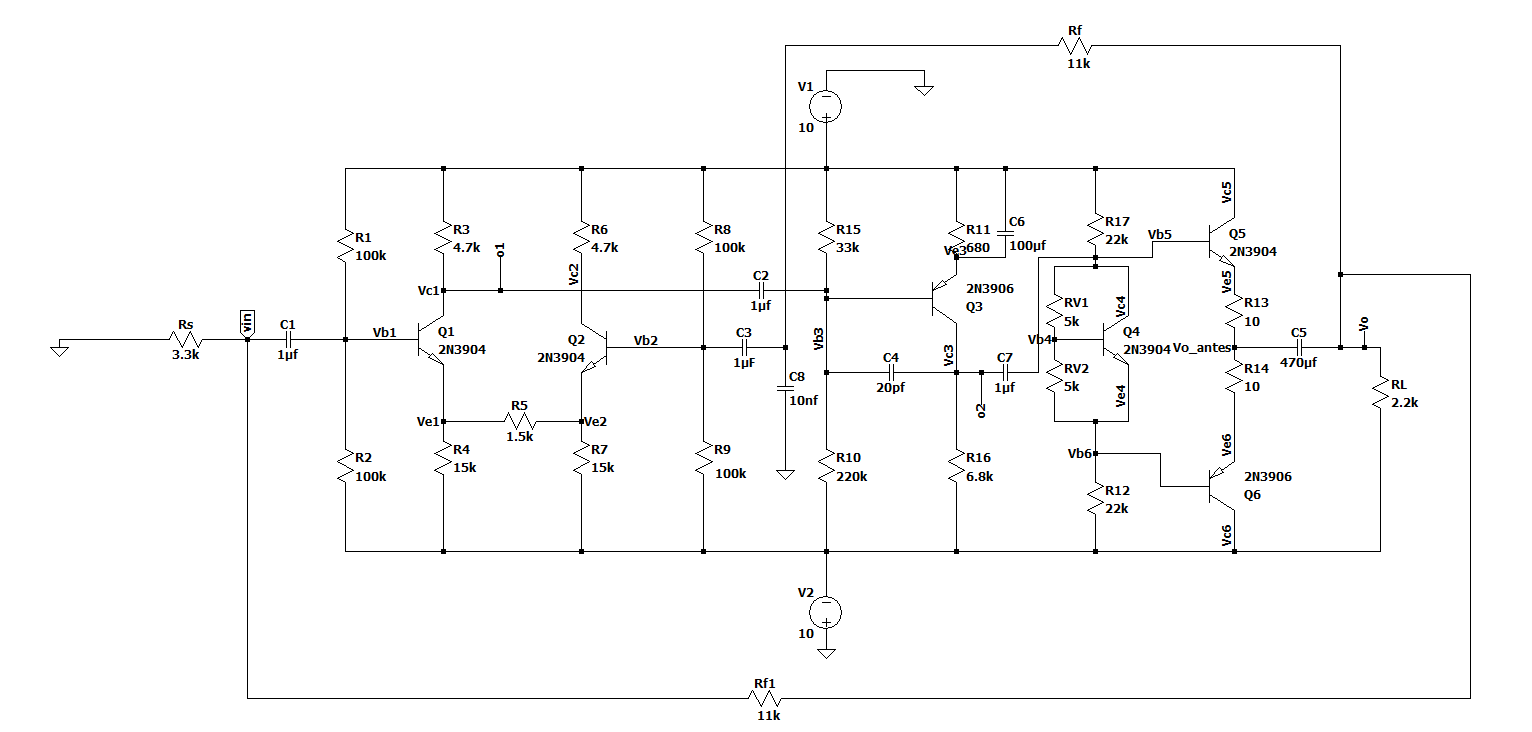
\includegraphics[width=\textwidth]{Imagenes/oscilador.png}
          \caption{Diagrama esquemático del amplificador base realimentado negativamente y positivamente.}
          \label{fig:oscilador}
        \end{figure}
        \subsubsection{Simulación}

  \item \textbf{Realice la simulación del circuito con el fin de verificar los cálculos previos.}
        \begin{itemize}
          \item \textbf{Realimentación negativa}



                \begin{figure}[H]
                  \centering
                  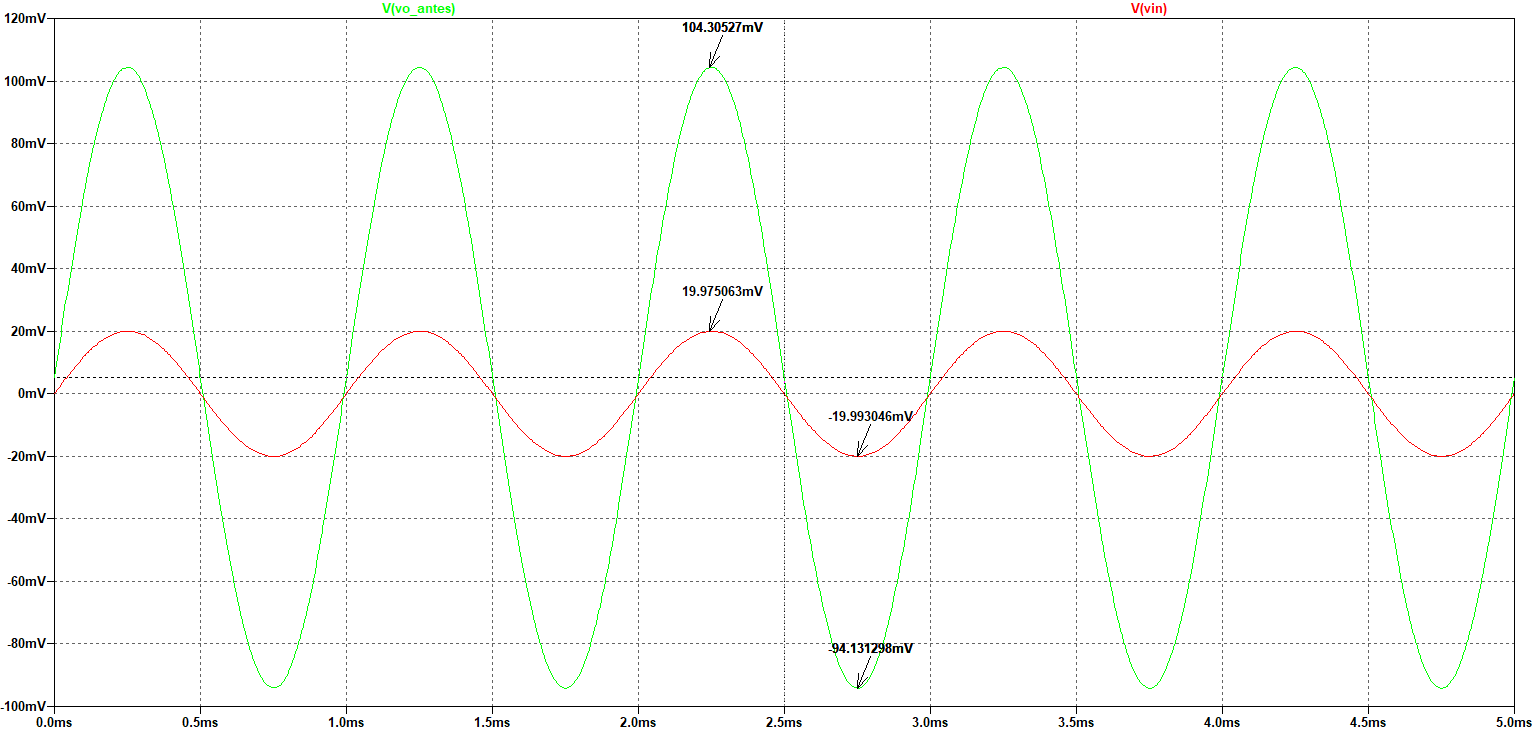
\includegraphics[width=\textwidth]{Imagenes/sim_vovi_realimentadon.png}
                  \captionsetup{labelfont={bf}}
                  \caption{Simulación del circuito de la figura \ref{fig:realimentadon}.}
                  \label{fig:sim_vovi_retroalimentadon}
                \end{figure}

                Si verificamos la ganancia de la realimentación negativa se tiene lo siguiente:

                \begin{align*}
                  A_{fb} & = \dfrac{104.30527m-(-94.131298m)}{19.975063m-(-19.993046m)} \\[0.2cm]
                  A_{fb} & = 4.965                                                      \\[0.2cm]
                \end{align*}

                Los valores son muy cercanos a los teóricos.

                \begin{figure}[H]
                  \centering
                  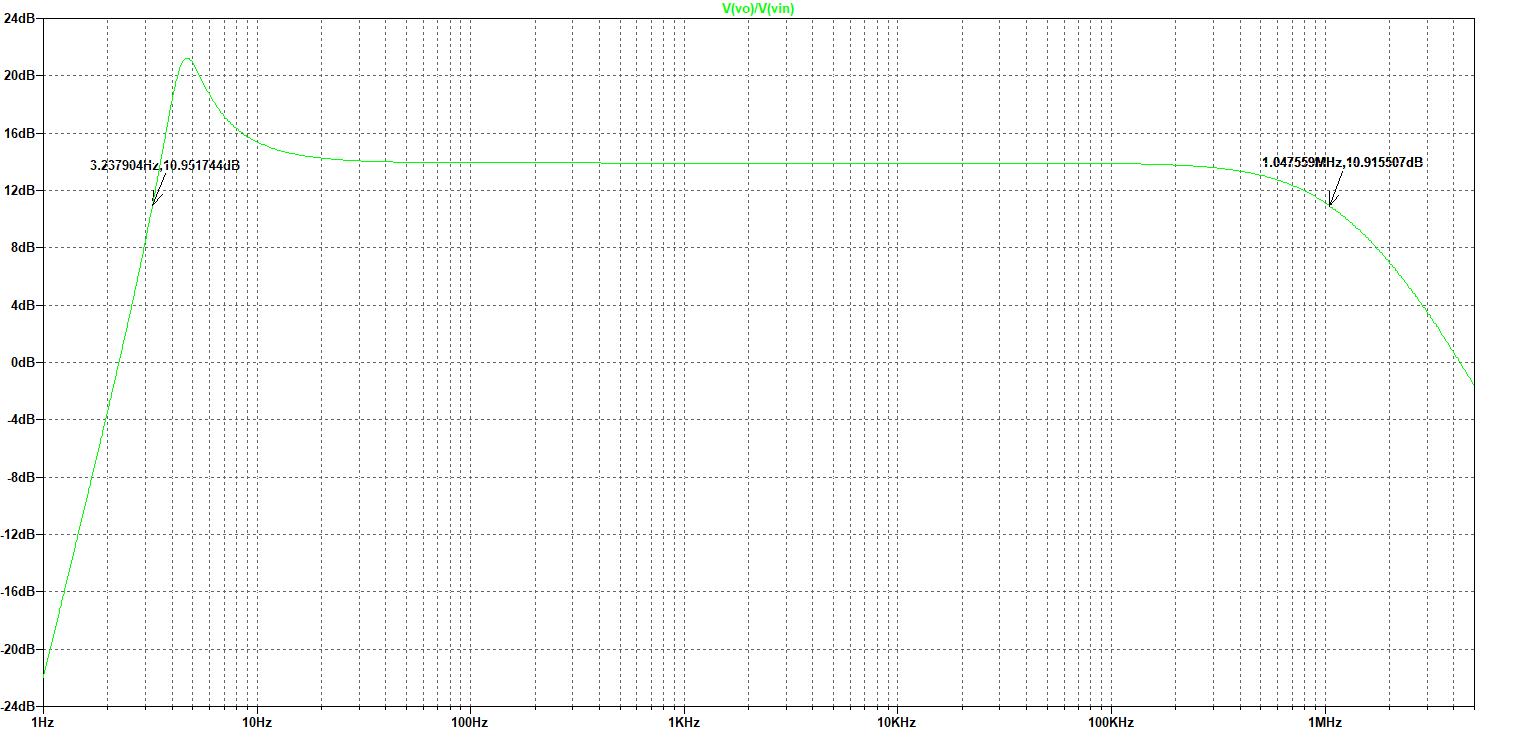
\includegraphics[width=\textwidth]{Imagenes/sim_resp_realimentadon.png}
                  \captionsetup{labelfont={bf}}
                  \caption{Simulación de la respuesta en frecuencia del circuito de la figura \ref{fig:realimentadon} .}
                  \label{fig:sim_resp_retroalimentadon}
                \end{figure}

                Son valores validos para los valores teóricos.

          \item \textbf{Realimentación negativa y positiva (oscilador)}


                \begin{figure}[H]
                  \centering
                  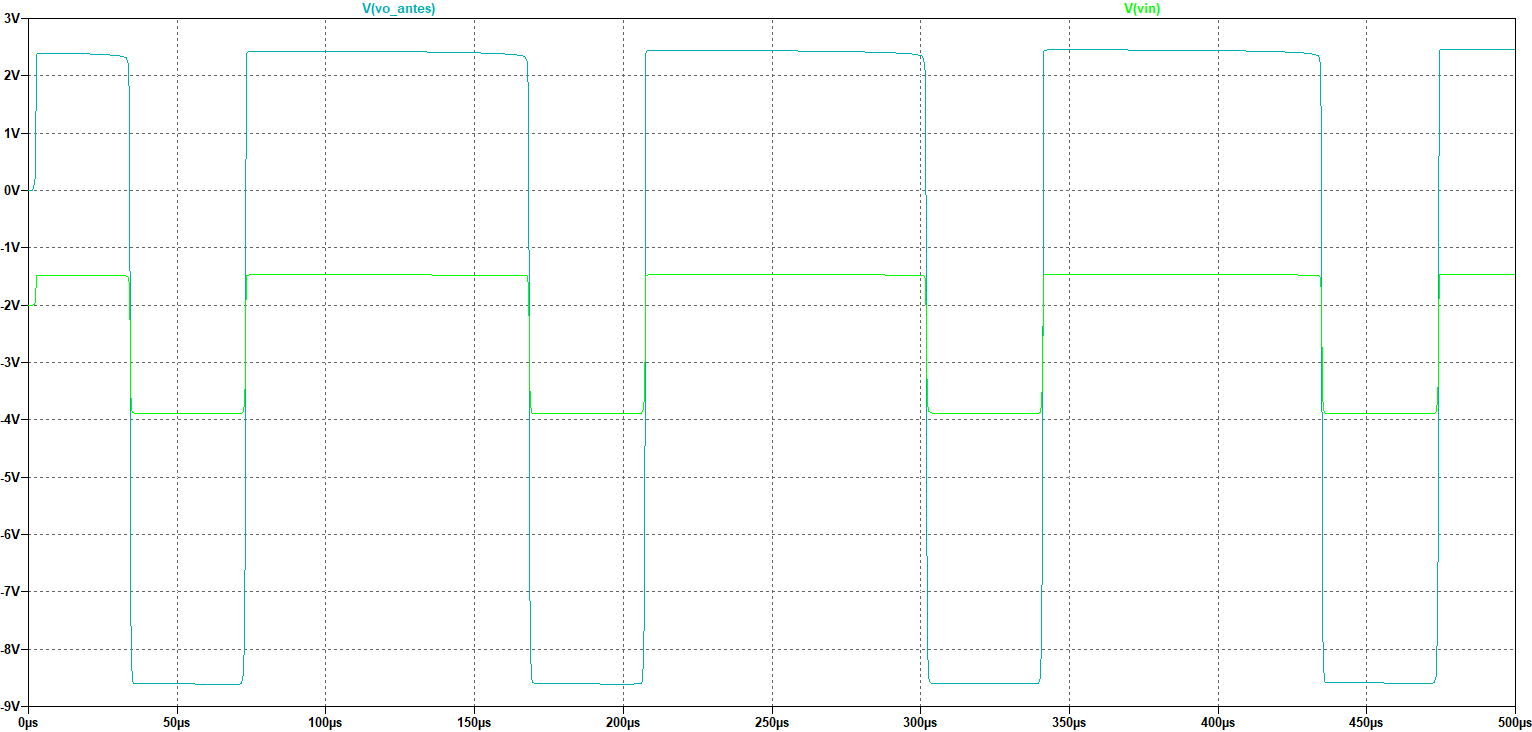
\includegraphics[width=\textwidth]{Imagenes/sim_oscilador.png}
                  \captionsetup{labelfont={bf}}
                  \caption{Simulación del circuito de la figura \ref{fig:oscilador}.}
                  \label{fig:sim_oscilador}
                \end{figure}

                Sin alimentación de entrada se observa sus oscilaciones por las realimentaciones debido a que este se convierte en un amplificador inestable por su realimentación positiva, sin embargo posee varias funcionalidades.
        \end{itemize}
\end{enumerate}








































































\newpage


